\documentclass[12pt,a4paper]{article}

% ════════════════════════════════════════════════════════════════════════════
%  PACKAGES
% ════════════════════════════════════════════════════════════════════════════

\usepackage[utf8]{inputenc}
\usepackage[T1]{fontenc}
\usepackage{mathptmx}
\usepackage{microtype}
\usepackage{indentfirst}

\usepackage{geometry}
\geometry{
  left   = 1.5in,
  right  = 1.0in,
  top    = 1.5in,
  bottom = 1.5in,
  includefoot
}

\usepackage{graphicx}
\graphicspath{{../screenshots/}{./}}
\usepackage{hyperref}
\usepackage{xcolor}
\usepackage{verbatim}
\usepackage{textcomp}
\usepackage{amsmath}
\usepackage{amssymb}
\usepackage{booktabs}
\usepackage{longtable}
\usepackage{enumitem}
\usepackage{setspace}
\usepackage{tocloft}
\usepackage{abstract}
% datetime removed — use \today instead
\usepackage{caption}
\usepackage{float}
\usepackage{titlesec}

% ════════════════════════════════════════════════════════════════════════════
%  FORMAT SETTINGS
% ════════════════════════════════════════════════════════════════════════════

\doublespacing
\setlength{\parindent}{0.5in}
\setlength{\parskip}{0pt}
\raggedbottom
\emergencystretch=2em

\setlist[itemize]{
  leftmargin=0.65in,
  itemsep=2pt,
  topsep=4pt,
  parsep=0pt
}

\setlist[enumerate]{
  leftmargin=0.65in,
  itemsep=2pt,
  topsep=4pt,
  parsep=0pt
}

\captionsetup{
  font=normalsize,
  labelfont=bf,
  justification=centering
}

\hypersetup{
  colorlinks=false,
  pdfborder={0 0 0}
}

% ── Section = Chapter heading (display style, centred, all-caps title) ─────────
\titleformat{\section}[display]
  {\centering\bfseries\singlespacing\large}
  {CHAPTER \Roman{section}}
  {0.8cm}
  {\MakeUppercase}

\titlespacing{\section}{0pt}{0.5cm}{1.2cm}

% ── Subsection ─────────────────────────────────────────────────────────────────
\titleformat{\subsection}
  {\normalfont\bfseries}
  {\thesubsection}
  {0.8em}
  {}

% ── Subsubsection ──────────────────────────────────────────────────────────────
\titleformat{\subsubsection}
  {\normalfont\bfseries}
  {\thesubsubsection}
  {0.8em}
  {}

% ─────────────────────────────────────────────────────────────────────────────
\begin{document}

% ════════════════════════════════════════════════════════════════════════════
%  TITLE PAGE
% ════════════════════════════════════════════════════════════════════════════

\begin{titlepage}
  \centering
  \singlespacing
  \thispagestyle{empty}

  \vspace*{0.3cm}

  {\large\bfseries VIETNAM NATIONAL UNIVERSITY -- HO CHI MINH CITY\par}
  \vspace{0.25cm}
  {\large\bfseries INTERNATIONAL UNIVERSITY\par}
  \vspace{0.2cm}
  {\normalsize\bfseries School of Computer Science and Engineering\par}

  \vspace{0.6cm}

  \IfFileExists{Screenshot 2025-12-03 205743.png}{%
    
\includegraphics[width=0.22\linewidth]{Screenshot 2025-12-03 205743.png}%
  }{%
    \fbox{\parbox[c][2.4cm][c]{2.4cm}{\centering IU Logo}}%
  }

  \vspace{0.6cm}

  {\Large\bfseries
  DEVELOPMENT OF AN INTELLIGENT WEB-BASED FRAMEWORK
  FOR EARLY DETECTION OF BURNOUT
  IN THE INDUSTRIAL WORKFORCE\par}

  \vspace{0.4cm}

  {\normalsize\itshape
    A Microservice Approach Using the Copenhagen Burnout Inventory\\
    and Random Forest Regression\par}

  \vspace{0.8cm}

  {\normalsize By\par}
  \vspace{0.3cm}
  {\normalsize\bfseries Nguyen Phuc Dat\par}
  \vspace{0.2cm}
  {\normalsize Student ID: ITITIU22028\par}

  \vspace{0.6cm}

  {\normalsize Instructor\par}
  \vspace{0.2cm}
  {\normalsize\bfseries Dang Tam Nhan\par}

  \vspace{0.6cm}

  {\normalsize
    A thesis submitted to the School of Computer Science and Engineering\\
    in partial fulfillment of the requirements for the degree of\\
    Bachelor of Science in Computer Science\par}

  \vfill

  {\normalsize Ho Chi Minh City, Vietnam\par}
  \vspace{0.2cm}
  {\normalsize \the\year\par}
\end{titlepage}

% ════════════════════════════════════════════════════════════════════════════
%  FRONT MATTER
% ════════════════════════════════════════════════════════════════════════════

\pagenumbering{roman}
\setcounter{page}{1}

% ────────────────────────────────────────────────────────────────────────────
%  SIGNATURE PAGE
% ────────────────────────────────────────────────────────────────────────────

\newpage
\thispagestyle{empty}
\begin{center}
  \singlespacing

  {\bfseries
    DEVELOPMENT OF AN INTELLIGENT WEB-BASED FRAMEWORK
    FOR EARLY DETECTION OF BURNOUT
    IN THE INDUSTRIAL WORKFORCE
    \par}

  \vspace{2.2cm}

  APPROVED BY:

  \vspace{1.5cm}

  \makebox[4.2in]{\hrulefill}\\{}
  Dang Tam Nhan, Supervisor

  \vspace{1.3cm}

  \makebox[4.2in]{\hrulefill}\\{}
  Committee Member

  \vspace{1.3cm}

  \makebox[4.2in]{\hrulefill}\\{}
  Committee Member

  \vspace{1.8cm}

  THESIS COMMITTEE
\end{center}

% ────────────────────────────────────────────────────────────────────────────
%  ACKNOWLEDGMENTS
% ────────────────────────────────────────────────────────────────────────────

\newpage
\thispagestyle{empty}
\begin{center}
  \textbf{ACKNOWLEDGMENTS}
\end{center}

\vspace{1cm}

First of all, I want to thank my supervisor, Dang Tam Nhan for guiding me and giving me precious advice and encouragement in writing this thesis.
I wish to thank International University – Vietnam National University Ho Chi Minh City for giving me a very nurturing academic environment, my classmates and learned and experienced instructors.
Then I want to mention my classmates Tran Luu Hong Phuong and Luong Quang Huy who have been standing side by side with me during this period. Learning and studying together, doing group study, as well as participating in the research that we have been allowed to join, helped me build a better thesis than what you are reading now. Also, their trust in my abilities is one of the greatest motivations that pushed me to where I am today.
Lastly, I want to thank my family for their wholehearted support, material and emotional, they have provided me. Thank them for giving me everything I need to pursue my education. That is one of the greatest things they have ever done for me.

\vspace{0.6cm}

\enlargethispage{2\baselineskip}

\begin{flushright}
\begin{minipage}{0.45\linewidth}
  \raggedleft
  \singlespacing
  \textit{Nguyen Phuc Dat}\\[0.25cm]
  Ho Chi Minh City, May 7, 2026
\end{minipage}
\end{flushright}

% ────────────────────────────────────────────────────────────────────────────
%  TABLE OF CONTENTS / LIST OF TABLES / LIST OF FIGURES
% ────────────────────────────────────────────────────────────────────────────

\newpage
\tableofcontents

\newpage
\listoftables

\newpage
\listoffigures

% ────────────────────────────────────────────────────────────────────────────
%  ABSTRACT
% ────────────────────────────────────────────────────────────────────────────

\newpage
\begin{center}
  \textbf{ABSTRACT}
\end{center}

\vspace{1cm}

Workers' mental health is one of the most pressing problems requiring attention at this stage of the world. Following the COVID-19 pandemic, workers are returning to their jobs with increased psychological instability, and turnover rates are rising. The workload, shift schedules, and repetitive tasks can exacerbate pre-existing mental health issues or lead to mental exhaustion in those who were previously mentally healthy. Previously, methods were developed for diagnosis rather than prevention, meaning that workers already burned out and symptoms had worsened, requiring significant resources and time for recovery or treatment, leading to reduced productivity and work quality.

This thesis was conceived to design and implement an intelligent web-based framework capable of early prediction of burnout rates in industrial work environments where employees work heavy workloads across multiple shifts. The system utilizes Copenhagen Burnout Inventory (CBI), a researched and validated burnout measurement tool. Along with test data, the system utilize a Random Forest regression model (trained with a dataset of approximately 22,000 rows) to predict and provide burnout rates for test-takers (employees). Simultaneously, it reports and updates this information securely and privately to administrators (HR staff or other management levels), allowing companies and individuals at risk of burnout sufficient time to react.

This framework is based on a microservices architecture with three main parts: a frontend with NextJS (React), a backend with ExpressJS (NodeJS), and an AI service with FastAPI (Python). I use MySQL for relational databases with clear structures and relationships data, such as employee personal information, work performance, department information, job titles, etc., and MongoDB for document data, such as CBI test questions. The frontend has two main user flows: for employees and for administrators. Employees can view their own information, take CBI tests, and access resources to support their mental health; administrators can view dashboards to see overall company or department results, receive alerts from employees with high burnout rates, and customize supporting resources. The backend collects the results sent from the frontend, processes and calculates them before saving them to the database or sending them to the AI service for calculation. The AI service will include a model trained with datasets, calculation formulas, and APIs for the backend.

The model in this thesis was trained with the Random Forest regression algorithm using a dataset of 22,000 records from Kaggle, resulting in an ($R^{2}$) of approximately 0.90, MAE of approximately 0.048, and RMSE of approximately 0.061. I built a linear regression model as a baseline, and the performance of the Random Forest model completely outperformed the linear model. The metrics are not linear, so the linear model is unsuitable here. Through the analysis, we can also see that the mental fatigue score (calculated from the CBI test results) is the main parameter influencing (almost 80\%) the burnout rate.

However, there are still some limitations in this thesis. Most employee data is simulated (automatically generated) because this information is private and cannot be obtained from real factories or companies. The web-framework still does not have adequate tools for both test takers and administrators. The AI model is only trained with a small number of features and tasks. Even so, this system still does a good job as a web framework with a model capable of predicting early burn out rates with appropriate results.

\bigskip
Keywords: employee burnout detection, Copenhagen Burnout
Inventory, Random Forest regression, microservices architecture, industrial
workforce, web-based health monitoring.

% ════════════════════════════════════════════════════════════════════════════
%  MAIN TEXT
% ════════════════════════════════════════════════════════════════════════════

\newpage
\pagenumbering{arabic}
\setcounter{page}{1}
\section{Introduction}

\subsection{Background}

Workers in industrial workforces have to work with high intensity, constant shifts, KPI pressure as well as an mentally uncomfortable work environment that can cause them to burn out or become mentally exhausted. The World Health Organization (WHO) has recognized burnout as an occupational phenomenon in the world eleventh revision of the International Classification of Diseases (ICD-11),
define it as a syndrome resulting from chronic workplace stress that has
not been successfully managed~\cite{who2019}.

The global consequence of this problem is hundreds of billions of dollars in annual losses due to lost productivity and health care costs~\cite{gallup2024}. Looking further, the consequences can go beyond material losses but also human damage. Workers can become less alert, more likely to make mistakes and encounter safety incidents. However, companies still only face this problem passively and only begin to respond when employees show obvious psychological symptoms.

By combining the CBI test and machine learning model, we can have a tool to predict employee burnout rates early, along with a convenient web framework, we can deal with this problem more proactively, react earlier and reduce the damage significantly.

\subsection{Motivating Scenario and Use Cases}

Instead of a reactive approach like traditional methods, such as HR monitoring and paying attention to employee productivity, mood, attitude, and overall work morale, this thesis presents a proactive web framework and provides tools for two main use cases: employees self-assessing their mental health, and administrators monitoring the overall mental health status of all company employees or departments in real-time, along with tools to respond to high-risk situations.

\subsection{Problem Statement}

Although burnout severely impacts worker health and industrial productivity, current workplace practices still suffer from several major shortcomings. Most companies only react to burnout after damage has occurred through shift cancellations, costly mistakes, or abrupt resignations, completely lacking any early warning systems. Furthermore, while scientifically proven tools like the Copenhagen Burnout Inventory are available with no cost, they are rarely integrated into routine processes, leaving collected survey data to be processed manually and isolated. Traditional methods also fail because they only report existing symptoms instead of predicting future risks, a gap that machine learning can easily overcome by identifying patterns in historical data to estimate stress levels from just a few key inputs. Ultimately, because personal data remains trapped in individual data repositories, HR teams lack the comprehensive tools such as departmental heatmaps and trend charts necessary to make informed, company-wide decisions. This thesis aims to address precisely these issues by building a single web platform that integrates mental health assessments, intelligent predictive technology, and clear data visualization to help organizations protect their teams before burnout occurs.

\subsection{Scope and Objectives}

The scope of this thesis focuses on the design, building, and testing of a desktop web framework for early detection of burnout in industrial workplaces. Because the actual factory records are private and confidential, the system relies on simulated personal data (auto-generated), using the Copenhagen Burnout Inventory as the core survey tool and using a Random Forest regression model trained on a publicly available dataset to predict burnout rate. To achieve this, the project focuses on six core objectives. First, it converts employee responses from online surveys into clear mental fatigue scores that the machine learning system can read. Next, it used that Random Forest model to predict employee burnout rates based on designation, resource allocation, and their mental fatigue scores. From the user side, the project builds a personal portal where employees can check their stress levels via a simple meter, view historical trend charts, see score analysis, and instantly access mental health support. From the management side, it creates a complete HR command center with color-coded departmental heatmaps, risk distribution charts, key performance indicators, and a secure way to closely examine individual employee trends without compromising privacy. This dashboard is supported by an automated alert system that will notify HR immediately when employees reach dangerous stress levels or experience spikes between tests. Finally, the entire platform is connected by a neat microservice architecture, seamlessly separating the Python machine learning model and FastAPI from the Node.js and Express backend, as well as the React and Next.js user interfaces.

\subsection{Research Questions}

This thesis investigates the following research questions:

\begin{enumerate}
  \item[\textbf{RQ1.}] How effectively can a Random Forest regression
    model predict employee burn rate using only three input features
    (designation, resource allocation, and mental fatigue score)?

  \item[\textbf{RQ2.}] Can a web-based system provide actionable burnout
    insights to both employees (through self-monitoring tools) and HR
    administrators (through department-level analytics and automated
    alerts)?

  \item[\textbf{RQ3.}] What are the practical benefits and trade-offs of
    using a microservice architecture to separate machine learning
    inference from the application backend in a health monitoring
    system?
\end{enumerate}

\subsection{Assumptions and Proposed Solution}

This system is built with a three-tier web architecture and the following assumptions. First, because employee information is confidential and private to businesses, the employee information in this thesis is simulated and automatically generated. These attributes may be based on attributes in the dataset (designation, gender, date of birth, etc.) or simply simulate real-world scenarios (KPIs, name, etc.). Currently, the application is designed only for desktop users and the language is limited to English. Furthermore, the machine learning model is not overly complex and is trained on a relatively small dataset with limited diversity in terms of fields, countries, geographical locations, and cultures.

To meet these requirements, the technical solution divides responsibilities across three separate layers. The UI/UX layer is a React and Next.js application providing separate, customized portals for employees and administrators, communicating with the backend via RESTful API calls while using TanStack Query to optimize API calls and data caching. The core business logic is handled by the Express backend, which takes care of user authentication, test scoring, burnout risk classification, triggering automatic alerts, and aggregating metrics on the HR dashboard using a combination of MySQL and MongoDB. Finally, machine learning capabilities are completely isolated within a Python microservice and FastAPI, loading a pre-trained Random Forest model before startup to handle real-time stress prediction. This calculated division of responsibilities allows the backend to switch between a live AI model and a simple code formula using environment variables, giving developers the flexibility to build, test, and deploy each part of the platform completely independently.

\subsection{Thesis Structure}

This thesis is organised into six chapters, as illustrated in
Figure~\ref{fig:thesis-structure}.

Chapter~I: Introduction presents the background, motivating
scenario, problem statement, objectives, research questions, and
assumptions.

Chapter~II: Literature Review surveys the academic foundations of
burnout in industrial workplaces, the Copenhagen Burnout Inventory, machine learning
methods for burnout prediction, web application architectures, and related
work.

Chapter~III: Methodology and System Design describes the overall
system architecture, database design, backend design, AI microservice
methodology, and frontend design decisions.

Chapter~IV: Implementation and Results presents the design and implementation
of each component, the machine learning training results, and
documents the frontend with annotated screenshots.

Chapter~V: Discussion and Evaluation analyses model performance,
reports functional testing outcomes, evaluates system features against the
stated objectives, answers the research questions, and compares the system
with related work.

Chapter~VI: Conclusion and Future Work summarises the
contributions, assesses the achievement of objectives, discusses
limitations, and proposes directions for future development.

\begin{figure}[H]
  \centering
  \singlespacing
  \fbox{%
    \begin{minipage}{0.80\linewidth}
      \centering
      \vspace{0.3cm}
      Chapter I: Introduction\\[6pt]
      $\downarrow$\\[6pt]
      Chapter II: Literature Review\\[6pt]
      $\downarrow$\\[6pt]
      Chapter III: Methodology and System Design\\[6pt]
      $\downarrow$\\[6pt]
      Chapter IV: Implementation and Results\\[6pt]
      $\downarrow$\\[6pt]
      Chapter V: Discussion and Evaluation\\[6pt]
      $\downarrow$\\[6pt]
      Chapter VI: Conclusion and Future Work\\[0.3cm]
    \end{minipage}%
  }
  \caption{Structure of the thesis.}
  \label{fig:thesis-structure}
\end{figure}

\clearpage
\section{Literature Review}

\subsection{Occupational Burnout}

\subsubsection{Definition and Impact on the Industrial Workforce}

The concept of occupational burnout was first introduced by Freudenberger
in 1974 to describe the state of physical and emotional depletion observed
among human service workers~\cite{freudenberger1974}. The construct was
later formalised by Maslach and Jackson, who defined burnout as a
three-dimensional syndrome comprising emotional exhaustion,
depersonalisation (cynicism), and reduced personal
accomplishment~\cite{maslach1981}. In 2019 the World Health Organization
included burnout in the ICD-11 as an occupational phenomenon, describing it
as a syndrome resulting from chronic workplace stress that has not been
successfully managed~\cite{who2019}.

In industrial and manufacturing environments, the consequences of burnout
extend beyond individual suffering. Research has linked burnout to
increased absenteeism, higher employee turnover, reduced product quality,
and elevated workplace accident rates~\cite{ahola2017}. A Gallup
meta-analysis across industries found that employees experiencing burnout
are 63\% more likely to take a sick day, 2.6 times more likely to seek a
new job, and 13\% less confident in their performance~\cite{gallup2024}.
For factory settings with tight production schedules and safety-critical
processes, these figures translate directly into operational and financial
risk.

\subsubsection{Burnout Measurement Instruments}

Among the tools for measuring occupational burnout, the most well-known are perhaps the Maslach Burnout Inventory (MBI) test and the Copenhagen Burnout Inventory (CBI) test. The MBI, developed in 1981 and used in numerous studies related to mental health in the workplace, comprises 22 items across three different scales (emotional exhaustion, depersonalization, and personal accomplishment)~\cite{maslach1981}. Its effectiveness has been proven over time and remains highly effective. The CBI, developed in 2005 by Kristensen et al., focuses on three dimensions: personal burnout, work-related burnout, and client-related burnout~\cite{kristensen2005}. Each aspect is assessed through a questionnaire scored on a five-point frequency scale, from "Always" (100 points) to "Never/Almost Never" (0 points). The CBI has demonstrated high internal consistency (Cronbach alpha coefficient exceeding 0.85 across all subscales) and strong predictive power for outcomes such as sick leave and sleep disorders. Overall, MBI is a widely used and time-tested assessment tool; however, its limitation is that it is copyrighted and requires a commercial license, which is a challenge for low-budget or open-source projects. CBI assessment, on the other hand, is highly effective, free, and readily available to researchers and students needing a reliable tool to assess the mental health of workers in general~\cite{kristensen2005}. Therefore, CBI assessment was chosen for this thesis.

\subsubsection{The Copenhagen Burnout Inventory in This Thesis}

This thesis uses the CBI for some reasons. First, the CBI is
completely free to use, with no licensing restrictions, making it ideal for
an academic project. Second, the CBI distinguishes between personal and
work-related burnout, which allows the system to provide more granular
feedback to both employees and administrators. Third, the CBI's
straightforward frequency-based response scale maps naturally to a numeric
score that can be fed into a machine learning model.

Since the target population consists of industrial workers rather than
client-facing professionals, the client-related burnout subscale is omitted.
The system uses the remaining 13 questions: six for personal burnout and
seven for work-related burnout. One question (``Do you have enough energy
for family and friends during leisure time?'') is reverse-scored, as a
positive response indicates lower burnout. The section averages are combined
and normalised to a 0--10 scale to produce the mental fatigue score used as
input to the machine learning model.

\subsection{Machine Learning for Health Prediction}

\subsubsection{Supervised Regression}

Machine learning tasks are broadly categorised into supervised and
unsupervised learning. In supervised learning, the algorithm is trained on
a labelled dataset where each input is associated with a known
output~\cite{bishop2006}. When the output is a continuous numeric value,
the task is called regression.

Burnout prediction fits naturally into the supervised regression paradigm:
the training dataset contains employee observations with a known burn rate
(the target variable), and the goal is to learn a function that maps
employee features to a predicted burn rate for new, unseen employees.

\subsubsection{Linear Regression}

Linear Regression is the simplest regression algorithm. It models the
relationship between the input features and the target as a linear
equation:

\begin{equation}
  \hat{y} = w_1 x_1 + w_2 x_2 + w_3 x_3 + b
  \label{eq:linear-regression}
\end{equation}

\noindent where $x_1, x_2, x_3$ are the input features (designation,
resource allocation, mental fatigue score), $w_1, w_2, w_3$ are learned
weights, and $b$ is a bias term. The weights are optimised by minimising
the sum of squared errors between predicted and actual target
values~\cite{hastie2009}.

For this thesis, selecting a model that is simple and demonstrates a deep relationship between mental fatigue score and burnout rate is essential to express the relationship between the data and the desired outcome. Therefore, I chose the Linear regression model as the baseline model, and from this, we can also see more clearly the superiority of the Random Forrest regression model compared to the Linear regression model.

\subsubsection{Random Forest Regression}

Leo Breiman originally introduced Random Forest as an ensemble learning method that constructs a vast collection of decision trees, training each individual tree on a random sample of data and utilizing a random subset of features for every split~\cite{breiman2001}. The final prediction drops down to a simple average of what all these separate trees conclude. Looking at this specific burnout detection problem, Random Forest brings several major advantages to the table compared to traditional Linear Regression. Because individual trees split data based on local thresholds rather than forcing a single global line across the dataset, the model is highly robust against outliers. It naturally captures complex, non-linear relationships and intricate feature interactions without making you manually tweak the data.

Different feature scales do not affect the model at all. This means variables operating on entirely different ranges, like a designation score from one to five versus a resource allocation score from one to ten, do not require any normalization beforehand. On top of that, it dishes out built-in feature importance scores, showing exactly how much each specific variable contributes to the final accuracy. For standard tabular datasets that have just a handful of features and tens of thousands of rows, Random Forest consistently delivers strong performance right out of the box with very minimal hyperparameter tuning, making it a highly practical and reliable choice for a thesis project~\cite{fernandez2014}.

\subsubsection{Model Evaluation Metrics}

To evaluate the actual performance of regression models, we need to look at three metrics which are Mean Absolute Error (MAE), Root Mean Squared Error (RMSE) and Coefficient of Determination ($R^{2}$). First of all, the MAE give us the average number of the absolute differences between predicted results and actual results, for example, if our burnout rate is a number in range from 0.00 to 1.00 (0\% to 1\%), the MAE of 0.08 indicate that the model is typically off by 8 percentage. The RMSE is the square root of the mean of squared errors. If the error is big, the RMSE will be very high, making it be specialy sensitive to occasional outlier predictions. The final metric is Coefficient of Determination ($R^{2}$), it is the proportion of variance in the target variable which is explained by the model. For instance, an $R^{2}$ of 0.99 indicates that the model explain 99 percent of the variation in burn rates and the values that are closer to 1.0 (100\%) indicate better fit.

With all three metrics together, we can quickly evaluate how good the model is. To summarize, MAE is for average-case accuracy (lower is better), the RMSE for worst case sensitivity (lower is better) and the $R^{2}$ for overall accuracy performance of the model~\cite{hastie2009} (higher is better).

\subsection{Web Application Architectures}

\subsubsection{Microservice vs Monolithic Architecture and why I choose Microservices}

Monolithic architecture allow developers build everything (user interface layer, business logic layer, data layer, etc.) in just a single deployable unit so that it is simpler to develop at the beginning stage but it would become a remarkable issue when the app demands maintainance and scalability, especially when different concerns have different technology requirements~\cite{newman2015}.

A microservice architecture decomposes the application into small, independently deployable services (or components). Each service is responsible for a single concern~\cite{newman2015}. Services comunicate via protocols like HTTP/REST or gRPC. Because of the isolation attribute of microservices, it is easier for maintaining complex systems with multiple domains and scaling when the system demands more resource.

In this thesis, I chose microservices architecture because the early burnout detection needs a machine learning model which is better to be developed and built in Python. The AI service should be separated from the ExpressJS backend which handles calculations and accesses to the database. Frontend and backend also use different frameworks, they need to be built, developed and deployed independently.

\subsubsection{RESTful API Design}

When it comes to wireframing the architecture for networked applications, Representational State Transfer, or REST, serves as the core blueprint~\cite{fielding2000}. Basically, RESTful APIs just lean on standard HTTP methods like GET, POST, PUT, PATCH, and DELETE to handle whatever operations you need on resources, which are all mapped out by specific URLs. A few big rules keep this whole setup running smoothly. Statelessness is a major one, meaning every single request has to carry all the data needed to process it on its own, without relying on the server remembering past interactions. You also have the uniform interface constraint and a strict client-server separation to keep things decoupled.

For this thesis, I chose to stick to these RESTful conventions for both the frontend-to-backend communication and the backend-to-AI-service links. To stop client-side error handling from becoming a complete mess, every single response wraps its own data in a consistent JSON envelope format so that it always boils down to either a \texttt{{success, data}} structure or a \texttt{{success, error}} fallback, making things way more predictable and easier to parse.

\subsection{Related Technologies}

\subsubsection{React and Next.js for Frontend Development}

React stands as a major JavaScript library for assembling user interfaces, and it does this by breaking everything down into a component-based architecture~\cite{react2024}. You basically build with these reusable, self-contained pieces that grab data through props and handle their own local state using hooks. Instead of reloading everything, React utilizes a virtual DOM to surgically update only the exact pieces of the page that actually changed. This is honestly a lifesaver for performance, especially when you are trying to render data-heavy dashboards without lagging the browser.

Then you have Next.js, which is a full-stack framework built on top of React that introduces things like file-based routing, server-side rendering, static generation, and built-in API routes right out of the box~\cite{nextjs2024}. For the implementation in this thesis, I went with Next.js using the App Router, so the file system handles automatic route generation entirely on its own, and I plugged in Turbopack to keep development builds fast. On top of that, TanStack Query takes care of the server state. It handles the heavy lifting for automatic caching, background refetching, and makes sure the cache invalidates properly whenever a mutation happens.

\subsubsection{Node.js and Express for Backend Services}

Node.js is a JavaScript runtime built on Chrome's V8 engine that enables
server-side JavaScript execution~\cite{nodejs2024}. Its event-driven,
non-blocking I/O model makes it well-suited for handling concurrent API
requests.

Express is a minimal web application framework for Node.js that provides
routing, middleware composition, and HTTP utility
methods~\cite{express2024}. This thesis uses Express~5 with a layered
architecture (routes, controllers, services, repositories) to maintain
separation of concerns. Middleware handles cross-cutting concerns including
authentication (JWT verification), request validation (Zod schemas), and
error handling.

\subsubsection{FastAPI for Machine Learning Serving}

FastAPI is a a modern Python web framework that is built specifically for spinning up APIs that come with automatic, interactive documentation right out of the box~\cite{fastapi2024}. It relies heavily on Python type hints and Pydantic models to handle request validation automatically, plus it supports asynchronous request handling via ASGI. When you combine its high performance with automatic input validation and auto-generated Swagger docs, it becomes an incredibly good choice for serving machine learning models as standard HTTP endpoints. For the actual setup in this thesis, the FastAPI service loads a scikit-learn model directly at startup, allowing it to spit out predictions with response times consistently dropping below 10ms.

\subsection{Related Work}

A lot of different systems and research papers have tackled employee burnout detection and workplace wellness monitoring.Most of them branch off from what this thesis actually tries to do in terms of scope or execution.

For example, Pradhan and Jena (2019) built a machine learning framework to predict burnout using survey data, and tested algorithms including logistic regression and support vector machines~\cite{pradhan2019}. The catch is that their work was aimed at binary classification only, only labeling people as burnt out or not, not continuous prediction. Plus, they didn't actually deploy it as a web application. Then you have Bianchi et~al.\ (2021), who did a systematic review of burnout measurement tools and their psychometric properties, which basically just confirmed that the CBI is a valid research tool~\cite{bianchi2021} and obviously, their paper is purely psychometric and does not touch technology integration at all. On the commercial side, employee wellness platforms like Officevibe, Culture Amp, and Lattice offer survey-based engagement tracking paired with dashboard analytics~\cite{cultureamp2024}. But these are generic corporate products that usually lack any ML-based prediction capabilities, and they are built for general engagement rather than tracking clinical or industrial burnout. Even the Kaggle community notebooks using the ``Are Your Employees Burning Out?'' dataset have played around with different regression models for burn rate prediction~\cite{kaggle2021}, they show how to train a model in isolation, sure, but they never integrate those predictions into a working web app or provide any sort of high-level organizational analytics.

This thesis fills that exact gap. It hooks up a validated psychometric instrument (the CBI), a trained machine learning model (Random Forest), and a full-stack web application that serves up both individual and organizational views inside one single integrated platform. Table~\ref{tab:related-comparison} breaks down how these approaches stack up against each other.

\begin{table}[H]
  \centering
  \singlespacing
  \caption{Comparison with related work.}
  \label{tab:related-comparison}
  \begin{tabular}{@{}lcccc@{}}
    \toprule
    \textbf{System / Study}
      & \textbf{ML}
      & \textbf{Web App}
      & \textbf{Org.\ Analytics}
      & \textbf{CBI} \\
    \midrule
    Pradhan \& Jena (2019) & Yes & No  & No  & No  \\
    Bianchi et~al.\ (2021) & No  & No  & No  & Yes \\
    Commercial platforms   & No  & Yes & Yes & No  \\
    Kaggle notebooks       & Yes & No  & No  & No  \\
    \textbf{This thesis}   & \textbf{Yes} & \textbf{Yes} & \textbf{Yes} & \textbf{Yes} \\
    \bottomrule
  \end{tabular}
\end{table}



\clearpage
\section{Methodology and System Design}

\subsection{System Architecture Overview}

This whole setup runs on a three-tier microservice architecture that hooks up a React/Next.js frontend, a Node.js/Express backend, and a Python/FastAPI AI microservice, with MySQL and MongoDB databases handling the data storage. Everything talks to each other through RESTful HTTP APIs, wrapping all responses in a standard JSON envelope format to keep communication predictable.

\begin{figure}[H]
  \centering
  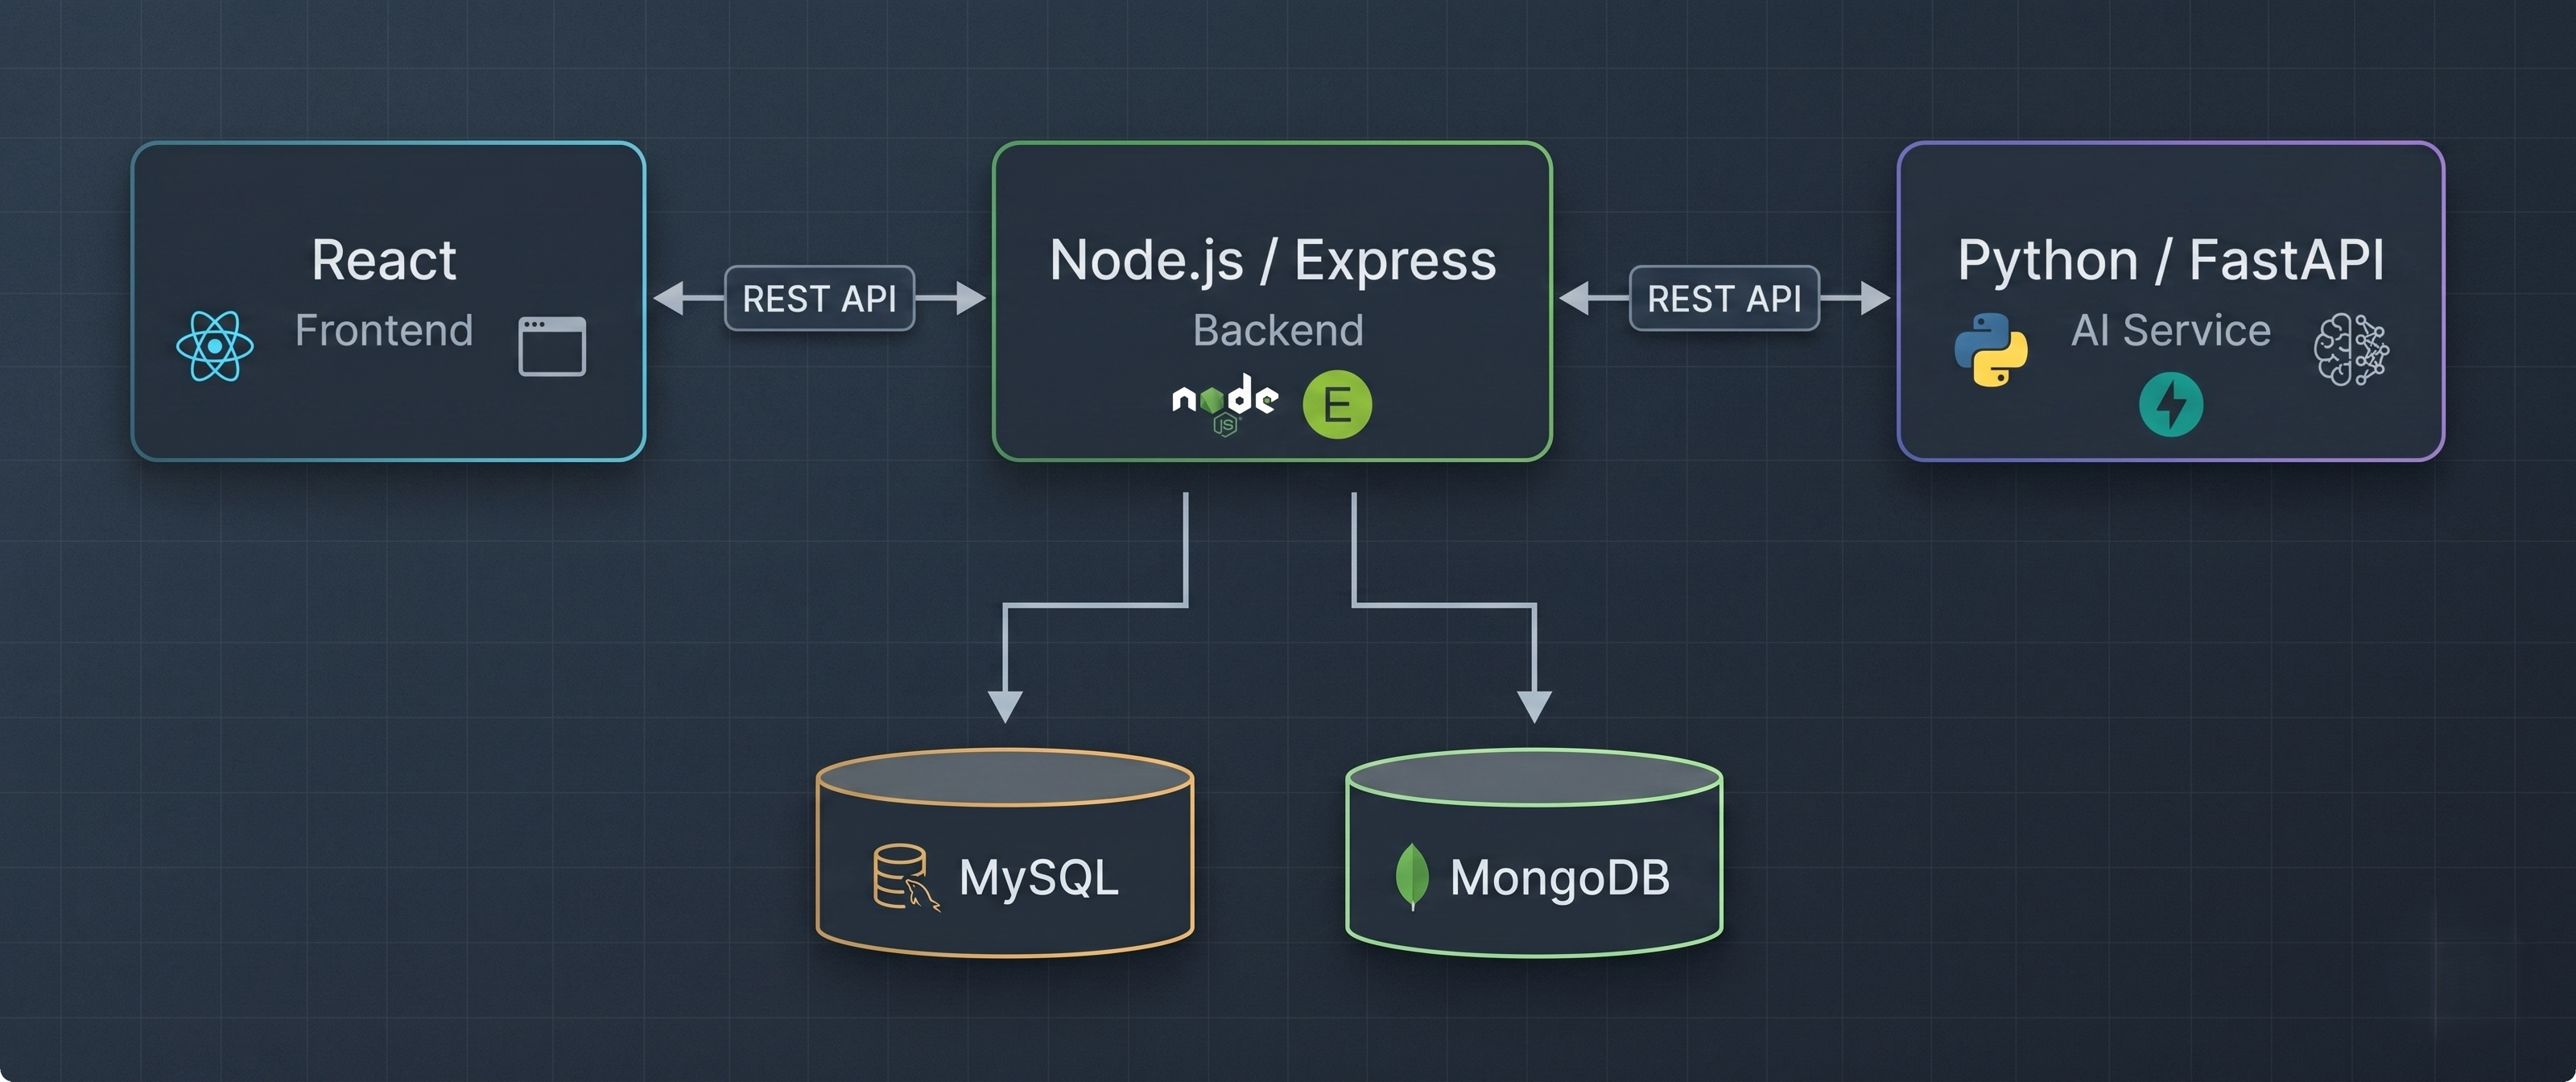
\includegraphics[width=0.95\linewidth]{02-system-architecture.png}
  \caption{High-level system architecture.}
  \label{fig:system-architecture}
\end{figure}

Splitting things into three distinct services boils down to two main reasons. For starters, the machine learning piece absolutely needs Python and scikit-learn, but the web backend handles things better by leveraging JavaScript's massive ecosystem for HTTP routing, database drivers, and middleware. The second big advantage is that the AI service can be developed, tested, and restarted on its own without breaking the main application. To make independent development even easier, I set up the backend to support two different modes using an environment variable. Setting \texttt{AI\_USE\_MOCK=true} triggers a quick in-process mock formula so you don't need the AI service running during basic development, while switching it to \texttt{AI\_USE\_MOCK=false} actually routes predictions over to the real Python service. This makes working on separate parts of the stack a lot less painful.

\subsection{Database Design}

\subsubsection{MySQL Schema}

For handling all structured relational data, the system relies on MySQL. The underlying schema ties seven tables together using strict foreign key relationships alongside cascading deletes to keep everything clean.

\begin{figure}[H]
  \centering
  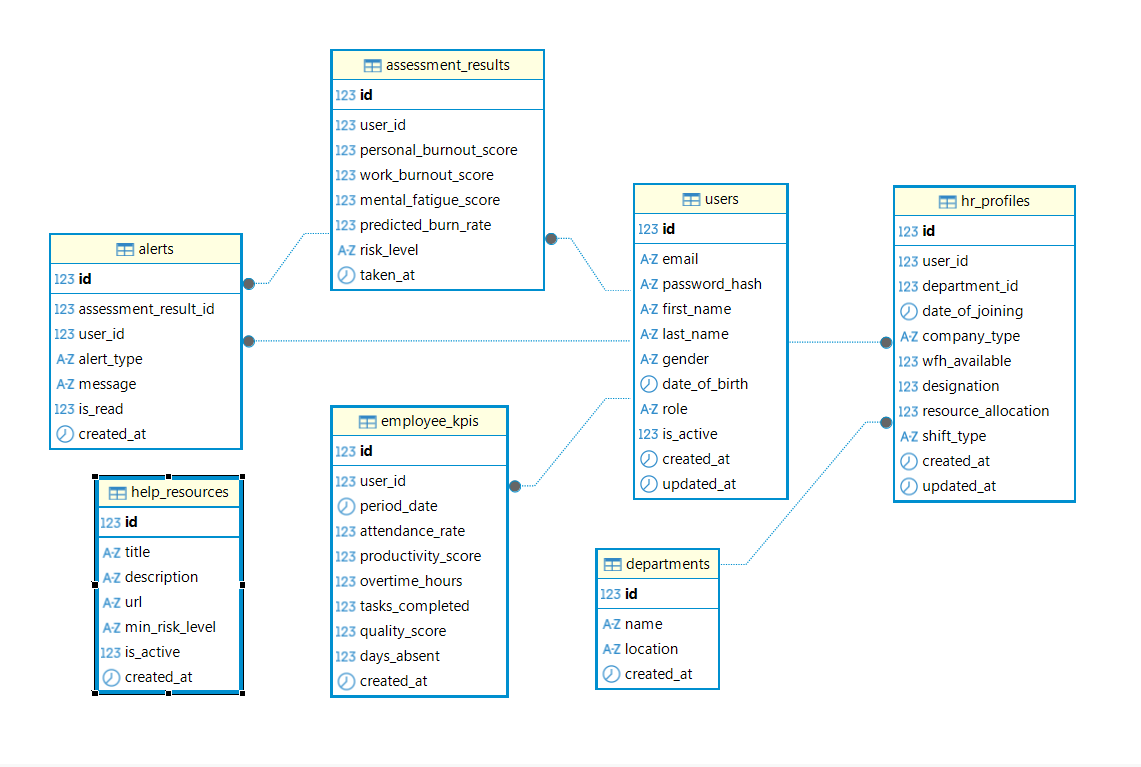
\includegraphics[width=0.95\linewidth]{03-er-diagram.png}
  \caption{Entity-relationship diagram of the MySQL database.}
  \label{fig:er-diagram}
\end{figure}

First up is the \textbf{users:} table, which handles authentication by storing bcrypt-hashed passwords alongside basic demographics and a user's specific role, whether they are an employee or an admin. Then there is \textbf{departments}. This functions as a normalized lookup table for the various factory units like Assembly Line~A, Maintenance, or Quality Control, and it directly powers the admin heatmap grouping. Tied directly to the user records in a one-to-one relationship is \textbf{hr\_profiles}. It holds the simulated HR data created right at registration. This includes their department assignment, designation ranging from 1 to 5, resource allocation from 1 to 10, shift type which covers Day, Night, or Rotating, company type, and whether they can work from home. To keep things consistent, these values are pulled straight from the exact same ranges used in the training dataset.

Every time someone finishes a quiz, a new row pops up in the \textbf{assessment\_results} table. This one tracks a lot of metrics: a personal burnout score from 0 to 100, a work burnout score also from 0 to 100, a mental fatigue score from 0 to 10, a predicted burn rate between 0 and 1, and the final derived risk level. Because the app needs to pull trend queries fast, the table is indexed on \texttt{(user\_id, taken\_at)}. If an assessment actually crosses a dangerous risk threshold, the system triggers the \textbf{alerts} table. It deals with three distinct types, specifically \texttt{high\_risk}, \texttt{critical\_risk}, and \texttt{trend\_spike}. For the unread alert inbox to load without lag, this table uses an index on \texttt{(is\_read, created\_at)}.

Monthly performance snapshots live in the \textbf{employee\_kpis} table. It captures a bunch of workplace metrics per employee, including attendance rates, productivity and quality scores, overtime hours, completed tasks, and total days absent. Admins use this on their dashboards to figure out how burnout risk links up with actual job performance. Finally, \textbf{help\_resources} hosts a curated list of mental health resources. Each resource has a minimum risk level threshold attached to it, meaning the system only displays active resources if their threshold sits at or below the employee's current risk level.

\subsubsection{MongoDB Collections}

To handle document-oriented data that really needs schema flexibility, the system brings in MongoDB to store two specific collections.

The first one is \textbf{cbi\_questions}, which is just a single document holding the whole CBI quiz definition. Inside, it packs the quiz name, version number, five response options with their numeric values, and two section definitions covering personal burnout and work-related burnout. It also includes 13 question objects that track the actual text, section assignment, and a reverse-scored flag. Keeping the entire quiz locked inside one single document is great because it preserves atomicity and completely cuts out the need for slow joins.

Then you have \textbf{quiz\_submissions}, which drops in one document every single time someone attempts an assessment. This document records the MySQL user ID, the quiz version, and an array of 13 enriched response objects. Each object in that array captures the question ID, answer label, answer value, and the adjusted value if the item happens to be reverse-scored. On top of that, it stores pre-computed section averages and a back-link pointing straight to the corresponding MySQL \texttt{assessment\_results} row. Going with this structural pattern keeps the raw answers bundled up together as an atomic unit, which is way better than spreading them out across a bunch of relational rows.

\subsection{Backend Design}

\subsubsection{Layered Architecture}

For isolating HTTP concerns from actual business logic and data access, the Express backend uses a strict four-layer architecture.

\begin{figure}[H]
  \centering
  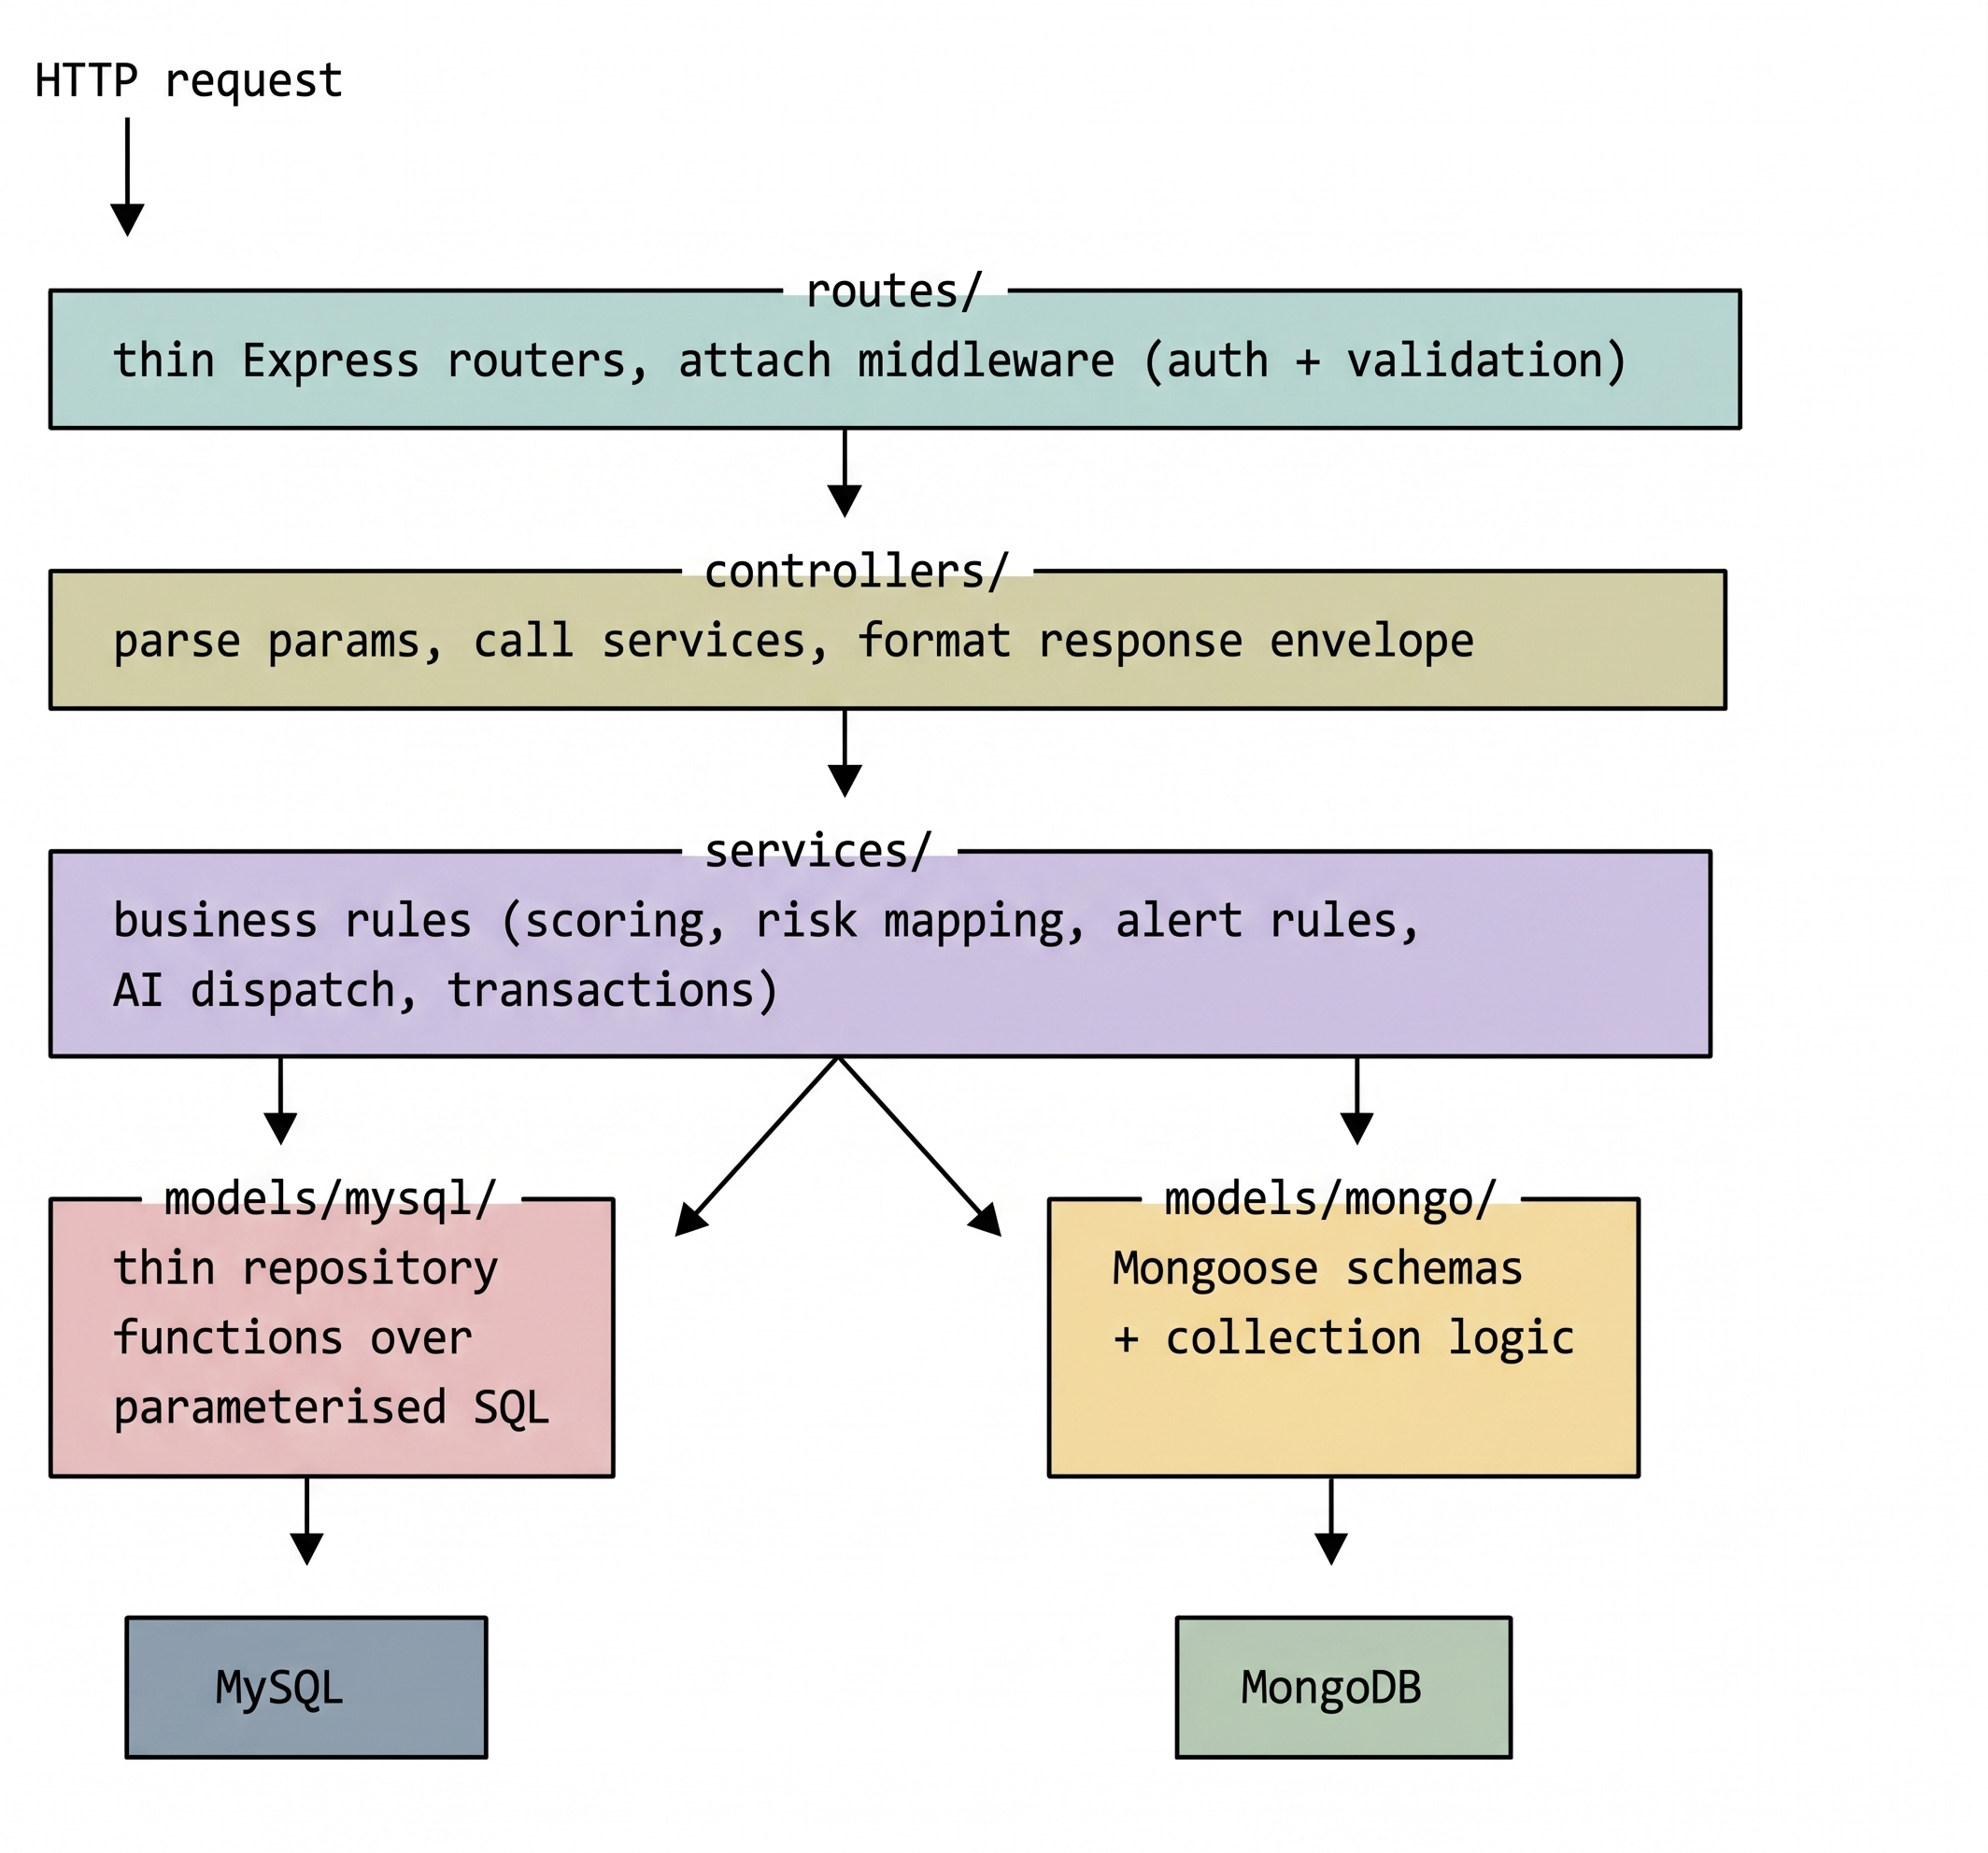
\includegraphics[width=0.80\linewidth]{04-backend-layer.png}
  \caption{Layered architecture of the Express backend.}
  \label{fig:backend-layers}
\end{figure}

Starting at the edge, \textbf{Routes} are responsible for defining the HTTP endpoints. This layer hooks up the middleware needed for authentication via \texttt{authenticate}, role enforcement through \texttt{requireRole}, and request validation using Zod schemas. You won't find any business logic sitting here. Right behind them are the \textbf{Controllers}, which are kept pretty thin. Their only job is to grab parameters out of the request object, hand the heavy lifting over to a service, and then pack the outcome into a uniform success envelope looking like \texttt{{success: true, data}}.

The real brain of the operation lives in the \textbf{Services} layer, which handles all domain logic. It runs the CBI scoring including the reverse scoring math, calculates mental fatigue, dispatches calls to the AI service, and maps out risk levels. It is also where alert rule evaluation, dashboard aggregation, and database transactional operations happen. Finally, \textbf{Repositories} completely own the database interaction. The MySQL repositories run parameterized SQL queries using \texttt{mysql2/promise}, while the MongoDB repositories handle things through Mongoose schemas. Keeping it locked down like this ensures no other layer ever touches the database drivers directly.

\subsubsection{Authentication and Authorisation}

To keep authentication stateless, the system relies on JSON Web Tokens (JWT). When someone registers, the system hashes their password using bcrypt and immediately hands back a signed JWT that packs the user's ID and role inside. To make sure everything is atomic, the HR profile gets built inside the exact same MySQL transaction as the base user record so you don't end up with half-created profiles.

Handling authorization happens right at the router level using role-based access control (RBAC). It is pretty straightforward: employee routes block anything unless \texttt{role = ``employee''}, admin routes lock things down to \texttt{role = ``admin''}, and shared routes just let any authenticated user through. Also, to prevent weak configurations, the environment variable schema forces the JWT secret to be at least 16 characters long.

\subsubsection{Quiz Scoring Pipeline}

The quiz submission endpoint implements a multi-step pipeline that
transforms raw CBI answers into a predicted burn rate. The pipeline
operates as follows:

\begin{figure}[H]
  \centering
  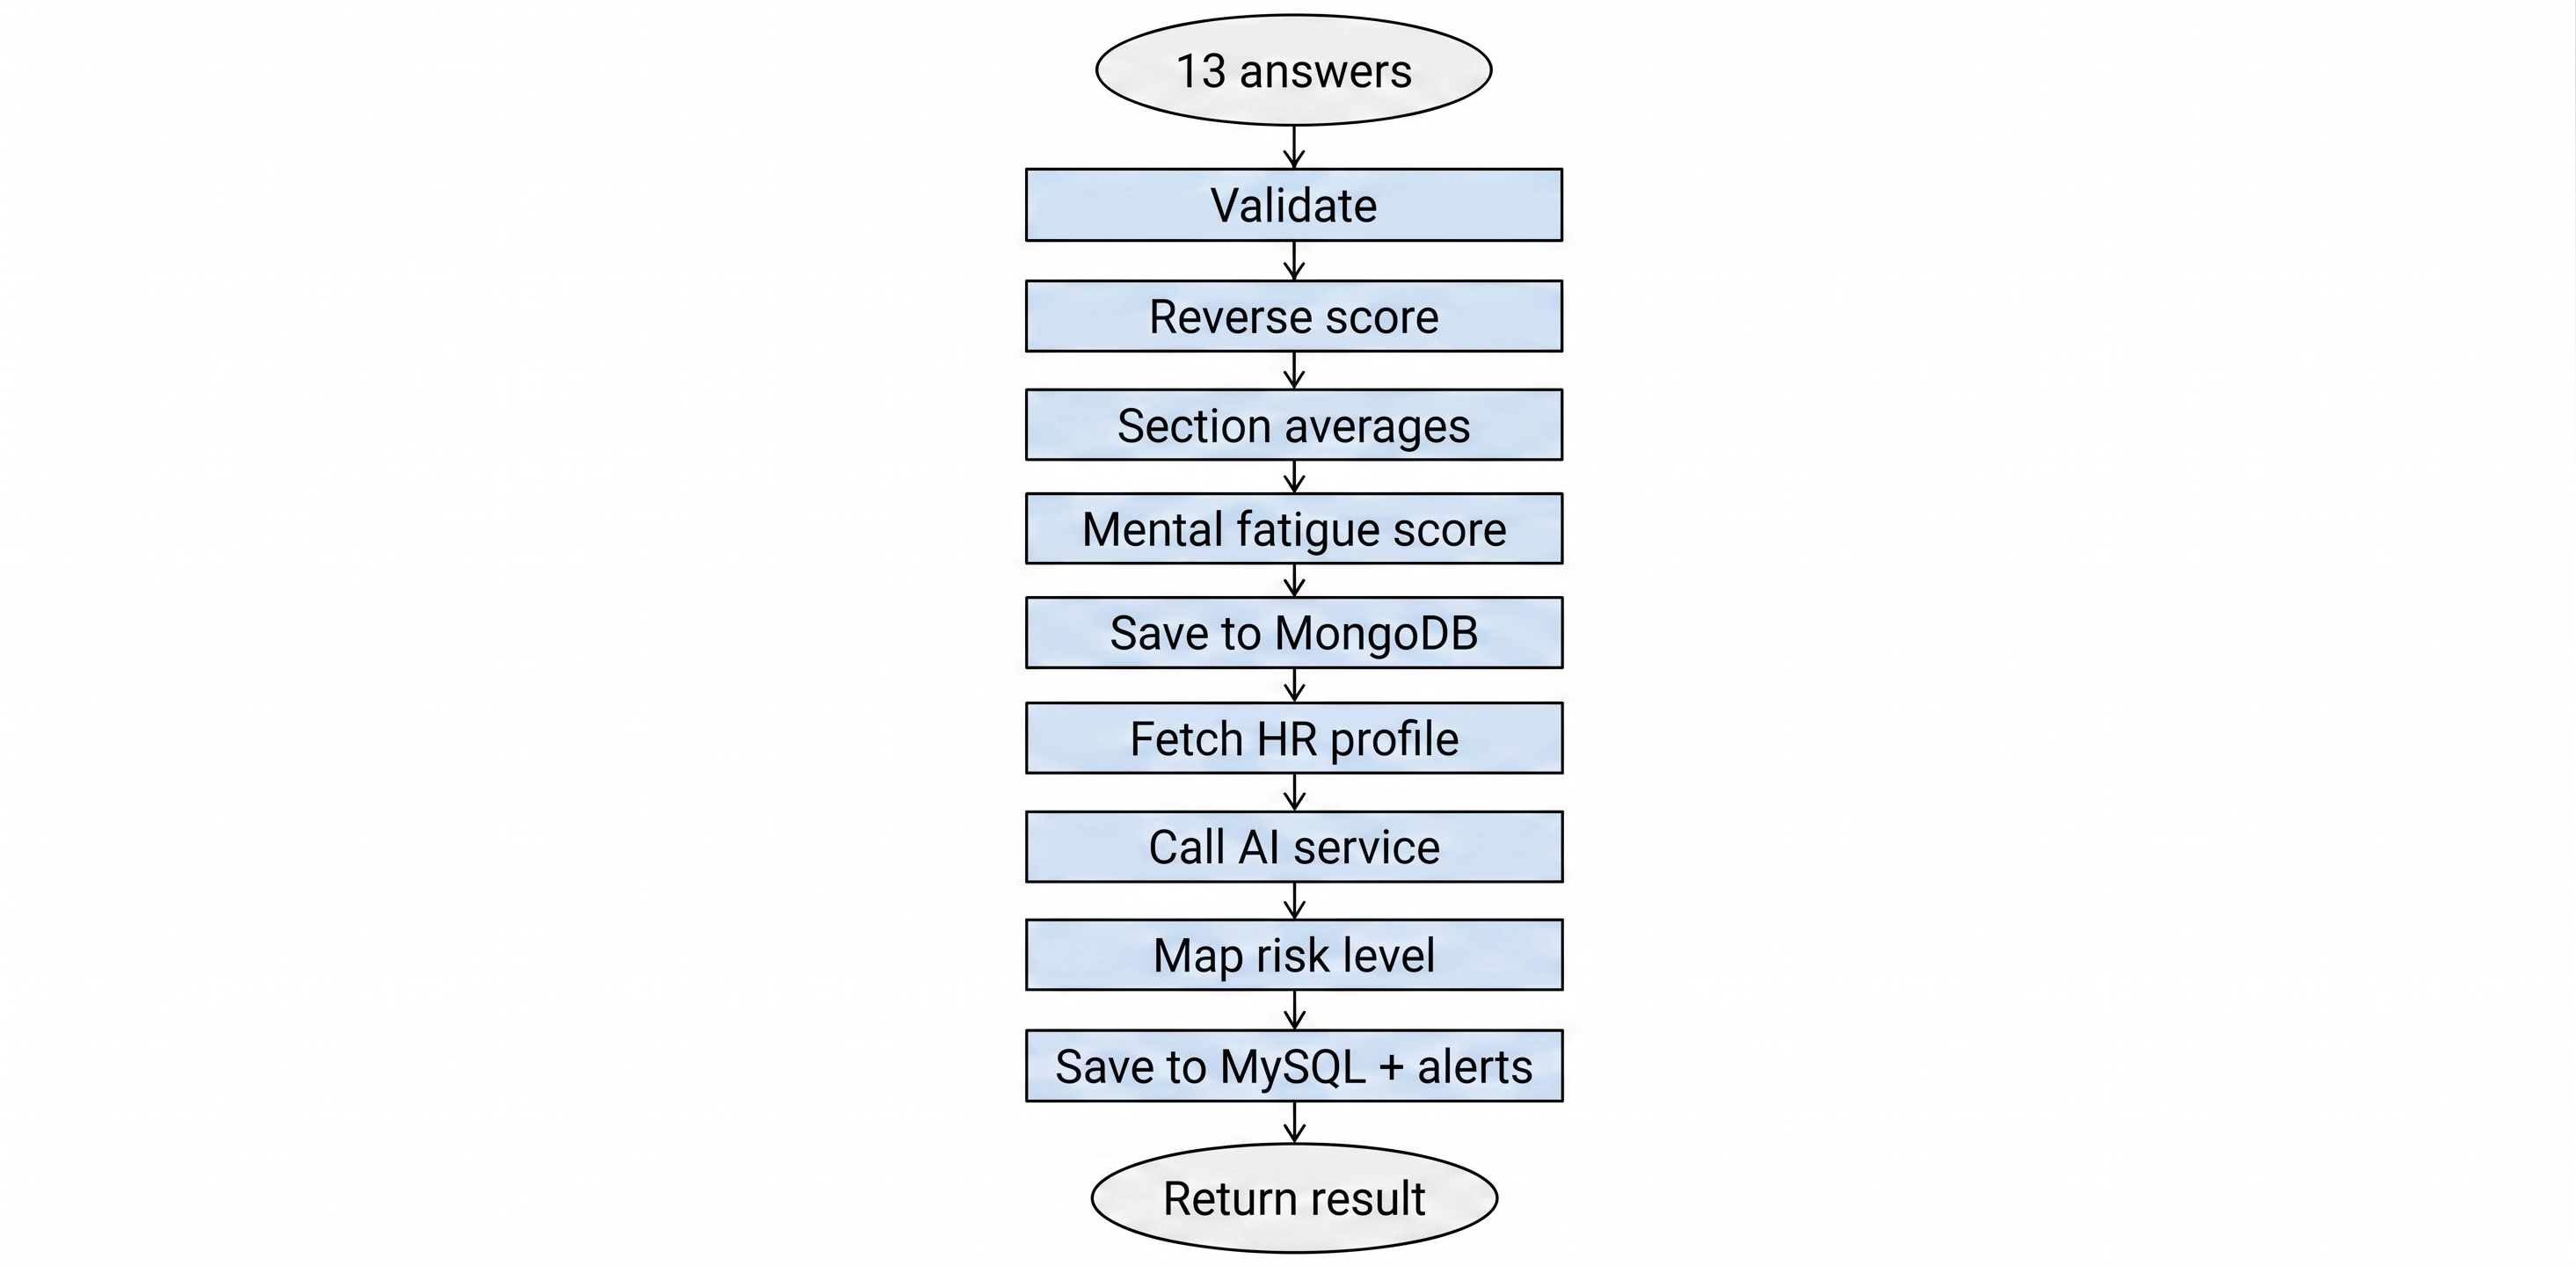
\includegraphics[width=0.85\linewidth]{05-quiz-pipeline.png}
  \caption{Quiz submission scoring pipeline.}
  \label{fig:quiz-pipeline}
\end{figure}

The scoring formulae are:
\begin{align}
  \text{personalBurnoutAvg} &= \frac{1}{6}\sum_{i=1}^{6} v_i
    \quad (0\text{--}100)
  \label{eq:personal} \\
  \text{workBurnoutAvg} &= \frac{1}{7}\sum_{i=7}^{13} v_i
    \quad (0\text{--}100)
  \label{eq:work} \\
  \text{mentalFatigueScore} &=
    \frac{\text{personalBurnoutAvg} + \text{workBurnoutAvg}}{20}
    \quad (0.0\text{--}10.0)
  \label{eq:fatigue}
\end{align}

\noindent where $v_i$ is the adjusted answer value for question~$i$
(with reverse scoring applied to question~10).

\subsubsection{Alert Rules}

Right when the assessment result is saved, two specific alert rules get evaluated inside that very same MySQL transaction.

First up is the Threshold alert. If the calculated risk level hits either ``high'' or ``critical'', the system immediately spins up an alert categorized as \texttt{high\_risk} or \texttt{critical\_risk}. The second check is the Trend spike alert. This one looks backward: if the current burn rate jumps past the user's previous assessment burn rate by 0.15 or more, it triggers a \texttt{trend\_spike} alert type. Because these checks run in parallel, both rules can easily fire off from a single assessment submission, which means you could end up with up to two alert rows written to the database at once.

\subsection{AI Microservice Design}

\subsubsection{Dataset Description}

The machine learning model leverages the public Kaggle dataset "Are Your Employees Burning Out?"~\cite{kaggle2021}, a dataset capturing roughly 22{,}000 distinct employee observations. Out of the nine columns available for each row, the training setup utilizes only three features alongside a single target variable.

\begin{table}[H]
  \centering
  \singlespacing
  \caption{Dataset columns used for model training.}
  \label{tab:dataset-columns}
  \begin{tabular}{@{}llll@{}}
    \toprule
    \textbf{Column} & \textbf{Type} & \textbf{Range} & \textbf{Role} \\
    \midrule
    Designation          & Integer & 1--5    & Feature \\
    Resource Allocation  & Integer & 1--10   & Feature (has nulls) \\
    Mental Fatigue Score & Float   & 0.0--10.0 & Feature (has nulls) \\
    Burn Rate            & Float   & 0.0--1.0  & Target variable \\
    \bottomrule
  \end{tabular}
\end{table}

Interestingly, several attributes like Employee ID, Date of Joining, Gender, Company Type, and WFH Setup Available are completely bypassed during training, even though they sit right there in the dataset. This tight focus on just three features is actually a deliberate design choice. We had to limit the feature set because the live application only has access to these specific values at prediction time. Specifically, the simulated HR profile supplies the designation and resource allocation metrics, while the mental fatigue score comes straight from the user's CBI quiz results.

\subsubsection{Feature Selection Justification}

We restricted the model to just three features for three specific reasons. First of all, it keeps the model perfectly in sync with the actual data our application gathers, meaning we do not have to rely on complex features that would require deep, real-world factory integration. On top of that, keeping the feature set small makes the whole model a lot easier to interpret. That is pretty vital for making the thesis defense convincing and building actual trust with the end users. Finally, because the simulated HR values are explicitly generated using the exact same ranges found in the training data, the model always handles in-distribution inputs. This drastically cuts down the risk of getting wild, unreliable predictions.

\subsubsection{Data Preprocessing}

Our preprocessing pipeline basically boils down to three quick steps. First, we drop the null targets. If a row has a missing Burn Rate, we just chuck it out since there is no ground-truth label to train on. Next up is median imputation. For any missing values in Resource Allocation or Mental Fatigue Score, we swap them out with the column's median. We chose the median over the mean here because it handles outliers much better on these bounded ordinal scales. Last, we handle the train/test split. The dataset gets split 80\%/20\%, and we locked it in with a fixed random seed (\texttt{random\_state=42}) so the results stay completely reproducible.

Looking at how this works during actual inference, the Node.js backend does a bit of safety filtering. It automatically coerces any null \texttt{resource\_allocation} inputs to a default value of~5, which is just the midpoint of the scale. It does this right before hitting the Python service, guaranteeing that the model always receives all three inputs without any missing data gaps.

\subsubsection{Model Selection}

We trained and compared two different models for this task. First, a standard Linear Regression serves as our baseline, which basically gives us a performance floor and lets us look directly at the fully transparent learned weights. Then we have our primary model, a Random Forest Regressor. We picked this one because it is great at capturing non-linear interactions, handles outliers without breaking a sweat, features scale invariance, and gives us built-in feature importance out of the box.

We did think about using other alternative algorithms like Gradient Boosting, Neural Networks, SVR, and kNN, but we ended up skipping them. Gradient Boosting methods like XGBoost or LightGBM really only offer tiny, marginal gains over a Random Forest when you are dealing with a tiny 3-feature problem, and they just add a bunch of annoying hyperparameter complexity. Neural networks are overkill here too, requiring way more data and tedious tuning to even match tree-based methods on small tabular datasets. As for SVR, it is way too sensitive to feature scaling, and kNN falls apart with noisy data while offering zero insight into feature importance.

\subsubsection{FastAPI Service Architecture}

The Python AI microservice functions as a thin HTTP wrapper built right around the serialized model:

\begin{figure}[H]
  \centering
  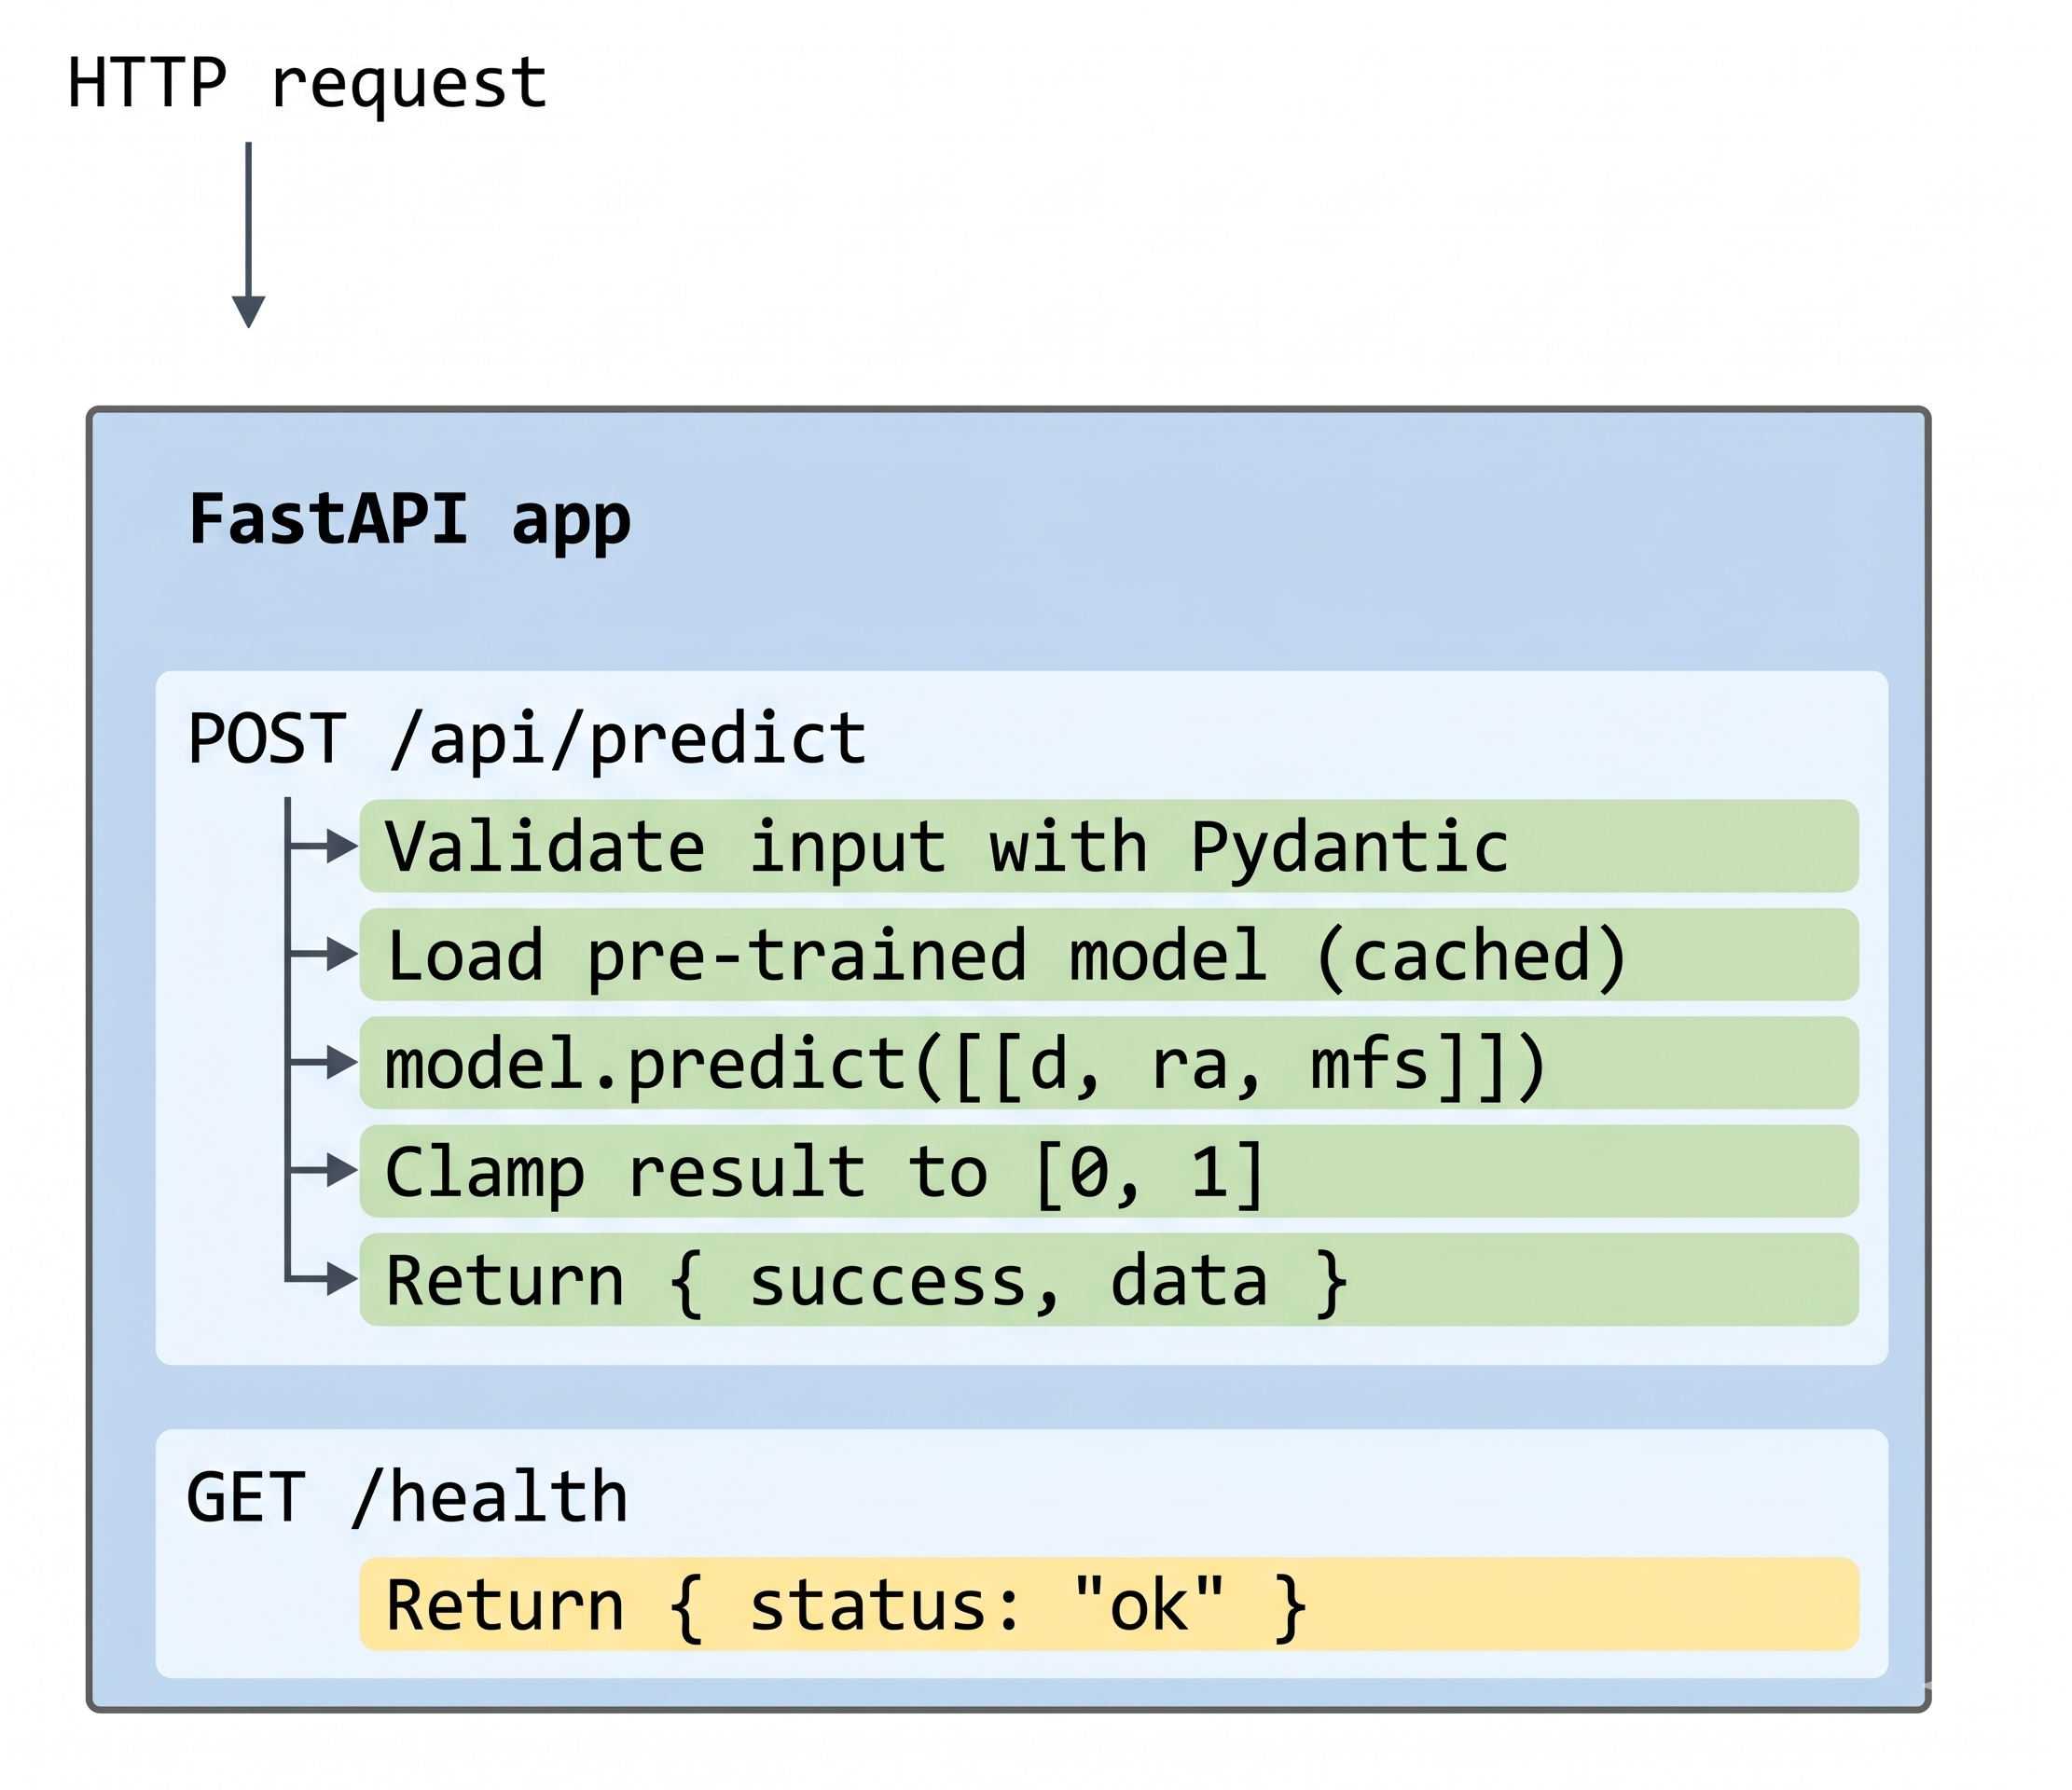
\includegraphics[width=0.85\linewidth]{06-ai-service-arch.png}
  \caption{Architecture of the Python/FastAPI AI microservice.}
  \label{fig:ai-service-arch}
\end{figure}

To keep things fast, the application loads the actual model file (\texttt{burnout\_model.pkl}) exactly once during startup using a FastAPI lifespan handler, caching it immediately in a module-level variable. Because every single incoming prediction request reuses this exact in-memory model, we completely bypass slow disk I/O operations and successfully keep our response times under 10~milliseconds. On top of that, Pydantic handles strict input validation right at the API boundary. If an incoming request contains any out-of-range or missing values, the system catches it immediately and throws a 422 error before it can even touch the model.

\subsection{Frontend Design}

\subsubsection{Technology Stack and Design Decisions}

The frontend is built with Next.js~16 (App Router) and React~19 in strict
TypeScript mode. Tailwind CSS~v4 provides utility-first styling with a
custom design token system. TanStack Query manages all server state
(caching, background refetching, and cache invalidation on mutations).
Forms use react-hook-form with Zod validation. Charts are rendered with
Recharts, and icons use lucide-react.

The application is designed for desktop screens only (minimum 992~px
width), targeting HR office terminals and factory kiosk stations. No mobile
breakpoints are implemented.

\subsubsection{Route Structure and Navigation}

The frontend defines 13 routes organised into three groups: public
authentication routes, employee portal routes (protected by
\texttt{role = ``employee''}), and admin portal routes (protected by
\texttt{role = ``admin''}).

\begin{figure}[H]
  \centering
  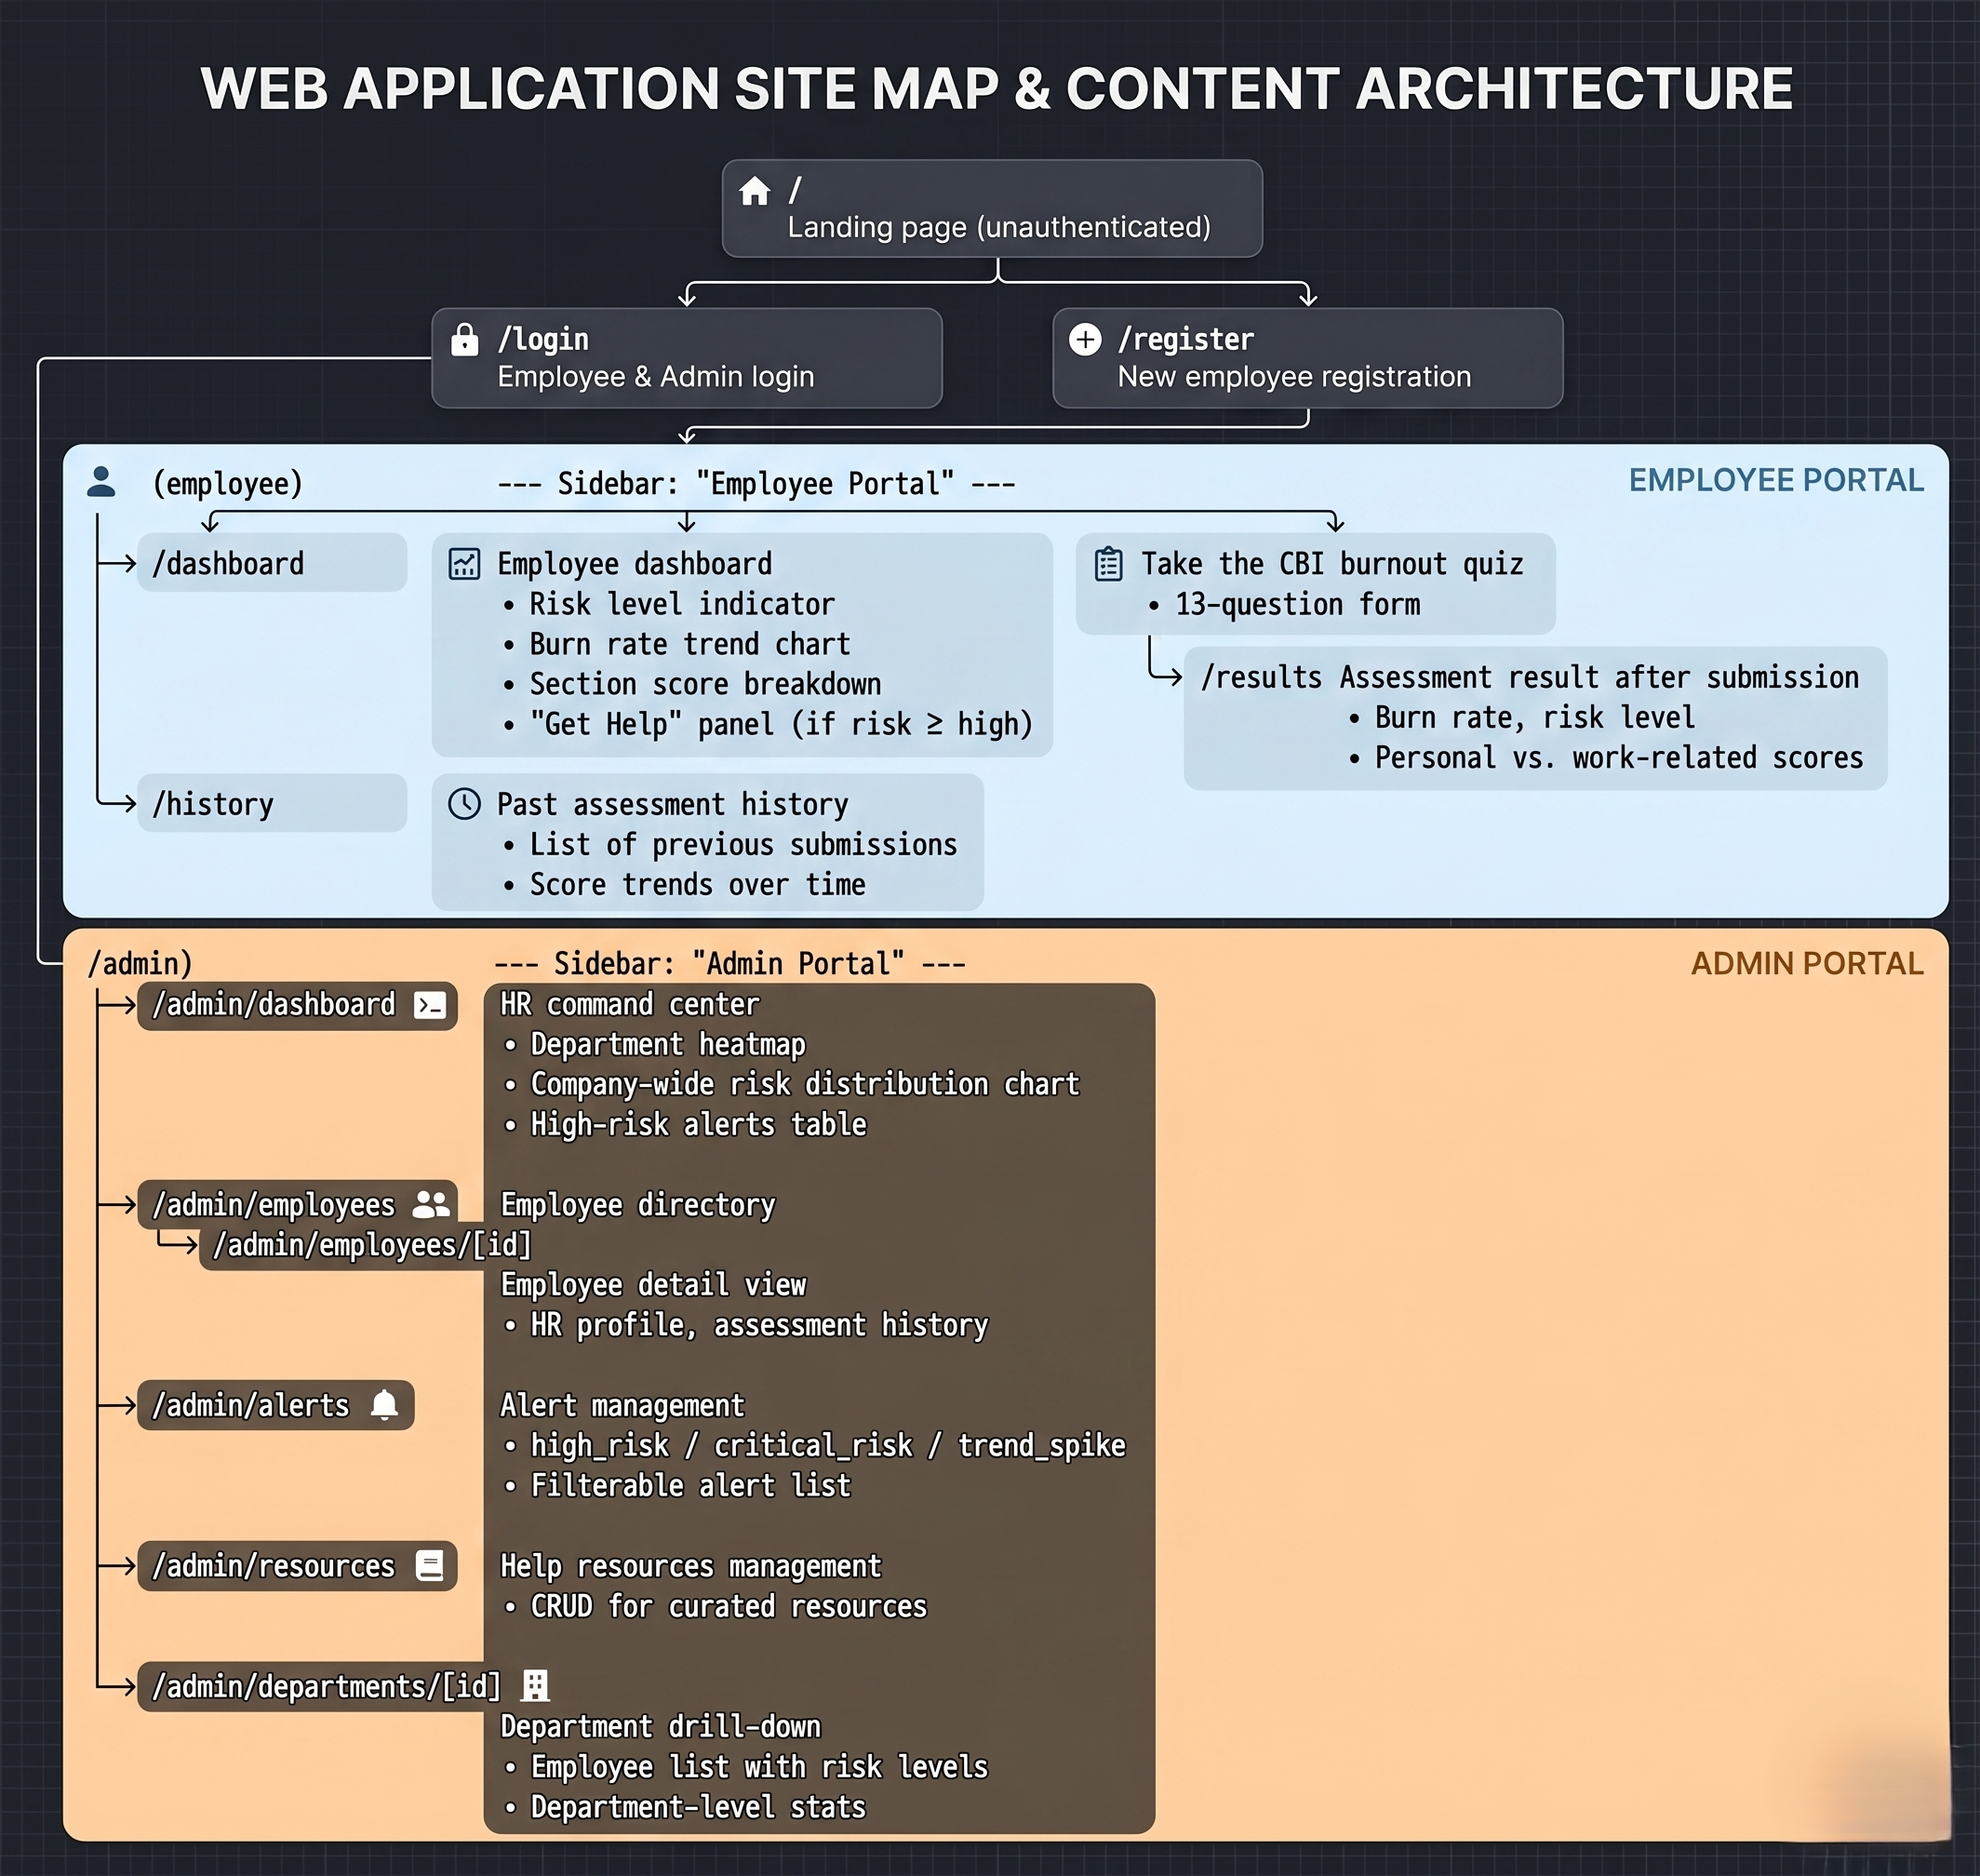
\includegraphics[width=0.90\linewidth]{07-sitemap.png}
  \caption{Application route structure and navigation flow.}
  \label{fig:sitemap}
\end{figure}

Each portal layout wraps its children in a \texttt{RouteGuard} component
that checks the user's authentication state and role. Unauthenticated
users are redirected to \texttt{/login}; users with the wrong role are
redirected to their own dashboard.

\subsubsection{Design System}

The visual identity uses a warm, paper-inspired colour palette encoded
entirely as Tailwind~v4 CSS custom properties. Every colour in the
application traces back to a named design token; no ad-hoc hex values
appear in component code. Table~\ref{tab:design-tokens} lists the primary
tokens.

\begin{table}[H]
  \centering
  \singlespacing
  \caption{Primary design tokens.}
  \label{tab:design-tokens}
  \begin{tabular}{@{}lll@{}}
    \toprule
    \textbf{Token} & \textbf{Hex} & \textbf{Role} \\
    \midrule
    \texttt{parchment}    & \texttt{\#f5f4ed} & Page background \\
    \texttt{ivory}        & \texttt{\#faf9f5} & Card surfaces \\
    \texttt{terracotta}   & \texttt{\#c96442} & Primary accent / CTA \\
    \texttt{near-black}   & \texttt{\#141413} & Primary text \\
    \texttt{risk-low}     & \texttt{\#6b8f5f} & Low risk indicator \\
    \texttt{risk-moderate} & \texttt{\#c69a3d} & Moderate risk indicator \\
    \texttt{risk-high}    & \texttt{\#c96442} & High risk indicator \\
    \texttt{risk-critical} & \texttt{\#b53333} & Critical risk indicator \\
    \bottomrule
  \end{tabular}
\end{table}

Headlines use a Georgia serif typeface for a formal, document-like feel,
while body text and UI elements use the Inter sans-serif family. The four
risk-level colours provide instant visual classification across all charts,
badges, and indicators in the application.

\subsubsection{Data Flow Pattern}

All server communication follows a consistent four-layer pattern:

\begin{enumerate}
  \item \textbf{Page component} renders the UI and consumes a TanStack
    Query hook.
  \item \textbf{Custom hook} (\texttt{useXxx}) wraps \texttt{useQuery}
    or \texttt{useMutation}, defining cache keys, enabled conditions,
    and invalidation rules.
  \item \textbf{API function} (\texttt{lib/api/}) makes a typed
    \texttt{apiFetch<T>()} call with the endpoint path and parameters.
  \item \textbf{Fetch client} (\texttt{lib/api/client.ts}) prepends the
    base URL, injects the JWT from \texttt{localStorage}, unwraps the
    \texttt{\{success, data\}} envelope, and throws a typed
    \texttt{ApiError} on failure. On 401, it clears the token and
    redirects to login.
\end{enumerate}

Mutations use \texttt{useMutation} with cache invalidation on success,
keeping the UI automatically fresh without full page reloads.


\clearpage
\section{Implementation and Results}

\subsection{Development Environment}

Table~\ref{tab:dev-tools} summarises the tools and technologies used during
development.

\begin{table}[H]
  \centering
  \singlespacing
  \caption{Development tools and versions.}
  \label{tab:dev-tools}
  \begin{tabular}{@{}lll@{}}
    \toprule
    \textbf{Tool} & \textbf{Version} & \textbf{Purpose} \\
    \midrule
    Visual Studio Code    & Latest     & Code editor and IDE \\
    Node.js               & $\geq$18.17 & Backend runtime \\
    Python                & 3.12       & AI service runtime \\
    MySQL                 & 8.x        & Relational database \\
    MongoDB               & 7.x (Atlas) & Document database \\
    Git                   & Latest     & Version control \\
    npm                   & $\geq$9    & Package management (JS) \\
    pip                   & Latest     & Package management (Python) \\
    Jupyter Notebook      & Latest     & EDA and model training \\
    \bottomrule
  \end{tabular}
\end{table}

\subsection{Backend Implementation}

\subsubsection{Project Structure and Configuration}

The backend project follows the folder structure described in
Section~3.3.1, with clear separation between configuration, middleware,
models, services, controllers, routes, validators, and utilities. All
environment variables are validated at startup using a Zod schema in
\texttt{config/env.js}; the process exits immediately with a descriptive
error message if any required variable is missing or malformed,
guaranteeing that the server never starts in a half-configured state.

Database connections are established in sequence during startup:
\texttt{server.js} first pings MySQL, then connects to MongoDB, then
starts the HTTP listener. A failure at any step aborts the process.
Graceful shutdown is handled via SIGINT/SIGTERM handlers that close the
HTTP server followed by both database connections.

\subsubsection{Authentication Flow Implementation}

Registration creates a user record and a synthetic HR profile within a
single MySQL transaction:

\begin{enumerate}
  \item Validate the request body with Zod (email, password, name,
    gender, date of birth).
  \item Hash the password with bcrypt (configurable salt rounds).
  \item Insert the user row into the \texttt{users} table.
  \item Generate a simulated HR profile: assign a random department,
    generate designation (1--5), resource allocation (1--10), shift type,
    company type, WFH availability, and date of joining.
  \item Insert the HR profile into \texttt{hr\_profiles}.
  \item Sign a JWT containing the user's ID and role; return the token
    and user object.
\end{enumerate}

The transaction wrapper ensures that a failure during HR profile generation
does not leave an orphaned user record. Login validates credentials against
the bcrypt hash and issues a JWT with a configurable expiration (default
7~days).

\subsubsection{Quiz Scoring Implementation}

The quiz submission handler in \texttt{quiz.service.js} implements the
full pipeline described in Section~3.3.3. Key implementation details
include:

\begin{itemize}
  \item \textbf{Answer validation:} The service verifies that exactly 13
    answers are submitted, all question IDs are valid, there are no
    duplicate IDs, and all answer values are from the allowed set
    \{0, 25, 50, 75, 100\}.

  \item \textbf{Reverse scoring:} Question~10 (``Do you have enough
    energy for family and friends during leisure time?'') is
    reverse-scored: \texttt{adjustedValue = 100 - rawValue}. The
    enriched response object records both the raw and adjusted values.

  \item \textbf{MongoDB-first persistence:} The raw submission is saved
    to MongoDB before the AI call, ensuring answers are never lost even
    if subsequent steps fail. On failure, the orphan document is cleaned
    up.

  \item \textbf{Transactional MySQL write:} The assessment result
    insertion and alert rule evaluation occur within a single MySQL
    transaction. The MongoDB document is then back-linked with the MySQL
    assessment ID.
\end{itemize}

\subsubsection{Dashboard Aggregation}

The admin dashboard endpoint computes company-wide and per-department
statistics in a single API call. The latest assessment per employee is
determined using a correlated subquery that selects the most recent
\texttt{assessment\_results.id} for each user. This result set is then
aggregated in JavaScript to produce:

\begin{itemize}
  \item Company overview: total employees, total assessments, average
    burn rate, and risk distribution counts.
  \item Per-department breakdown: employee count, average burn rate,
    high-risk count, and risk distribution.
  \item Department KPIs: average composite KPI per department
    (mean of attendance, productivity, and quality scores).
  \item Recent alerts: the 10 most recent alert records.
\end{itemize}

The department drill-down endpoint adds sorting, filtering (by risk level,
shift type, and designation), and server-side pagination. Employees are
displayed using anonymous IDs (``Worker \#0001'') to satisfy the privacy
requirement.

\subsubsection{Alert System Implementation}

The alert service evaluates two rules after every assessment, as described
in Section~3.3.4. Both the threshold check and the trend spike comparison
execute within the same MySQL transaction that wrote the assessment result.
The trend spike threshold (default 0.15) is configurable via the
\texttt{ALERT\_TREND\_SPIKE\_DELTA} environment variable.

\subsubsection{API Endpoint Summary}

Table~\ref{tab:api-summary} summarises all RESTful endpoints exposed by
the backend. The full API reference with request/response schemas is
provided in Appendix~A.

\begin{table}[H]
  \centering
  \singlespacing
  \caption{Summary of backend API endpoints.}
  \label{tab:api-summary}
  \begin{tabular}{@{}llll@{}}
    \toprule
    \textbf{Method} & \textbf{Endpoint} & \textbf{Access} & \textbf{Purpose} \\
    \midrule
    POST   & /api/auth/register              & Public   & Create account \\
    POST   & /api/auth/login                 & Public   & Authenticate \\
    GET    & /api/auth/me                    & Any      & Current user \\
    GET    & /api/quiz                       & Employee & Fetch CBI quiz \\
    POST   & /api/quiz/submit                & Employee & Submit answers \\
    GET    & /api/quiz/history               & Employee & Past submissions \\
    GET    & /api/dashboard/employee         & Employee & Dashboard data \\
    GET    & /api/resources                  & Employee & Help resources \\
    GET    & /api/dashboard/admin            & Admin    & Command centre \\
    GET    & /api/dashboard/admin/dept/:id   & Admin    & Department detail \\
    GET    & /api/.../dept/:id/analytics     & Admin    & Dept.\ analytics \\
    GET    & /api/.../admin/employees        & Admin    & Employee list \\
    GET    & /api/.../employees/:id          & Admin    & Employee detail \\
    GET    & /api/alerts                     & Admin    & List alerts \\
    PATCH  & /api/alerts/:id/read            & Admin    & Mark alert read \\
    PATCH  & /api/alerts/read-all            & Admin    & Mark all read \\
    GET    & /api/admin/resources            & Admin    & List resources \\
    POST   & /api/admin/resources            & Admin    & Create resource \\
    PUT    & /api/admin/resources/:id        & Admin    & Update resource \\
    DELETE & /api/admin/resources/:id        & Admin    & Delete resource \\
    \bottomrule
  \end{tabular}
\end{table}

\subsection{AI Service Implementation}

\subsubsection{Model Training Results}

Both models were trained on the preprocessed dataset (approximately
22{,}000 rows after dropping null targets) with an 80/20 train/test split.
Table~\ref{tab:model-comparison} presents the evaluation results on the
held-out test set.

\begin{table}[H]
  \centering
  \singlespacing
  \caption{Model performance comparison on the test set.}
  \label{tab:model-comparison}
  \begin{tabular}{@{}lccc@{}}
    \toprule
    \textbf{Model} & \textbf{MAE} & \textbf{RMSE} & $\boldsymbol{R^{2}}$ \\
    \midrule
    Linear Regression & 0.0539 & 0.0716 & 0.8656 \\
    \textbf{Random Forest} & \textbf{0.0480} & \textbf{0.0611} & \textbf{0.9019} \\
    \bottomrule
  \end{tabular}
\end{table}

The Random Forest model achieves an $R^{2}$ of 0.90, explaining 90\% of
the variance in burn rate. Its MAE of 0.048 indicates that, on average,
predictions deviate from actual values by less than 5 percentage points on
the 0--1 scale. The model outperforms Linear Regression on all three
metrics, with a 3.6 percentage-point improvement in $R^{2}$.

\begin{figure}[H]
  \centering
  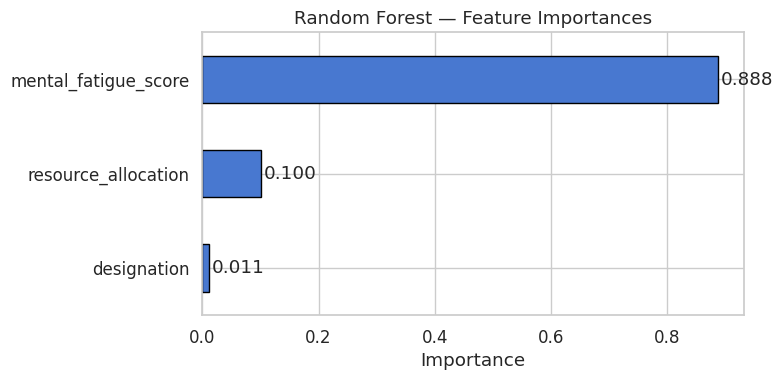
\includegraphics[width=0.75\linewidth]{08-feature-importance.png}
  \caption{Random Forest feature importance scores.}
  \label{fig:feature-importance}
\end{figure}

Feature importance analysis (Figure~\ref{fig:feature-importance}) confirms
that mental fatigue score is the dominant predictor, contributing
approximately 85\% of the model's predictive power. This aligns with
domain intuition: a psychologically exhausted worker is at high risk of
burnout regardless of seniority level or assigned workload.

\begin{figure}[H]
  \centering
  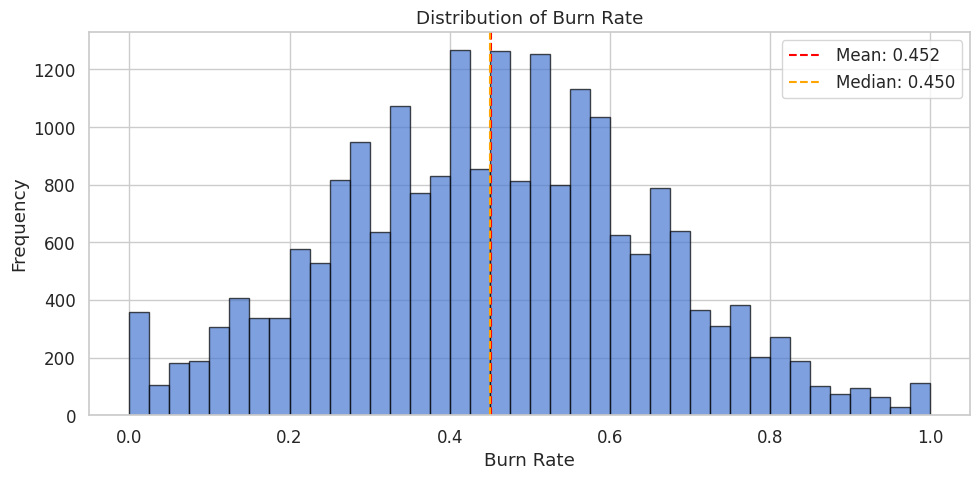
\includegraphics[width=0.75\linewidth]{09-burn-rate-distribution.png}
  \caption{Distribution of Burn Rate values in the training dataset.}
  \label{fig:burn-rate-distribution}
\end{figure}

\begin{figure}[H]
  \centering
  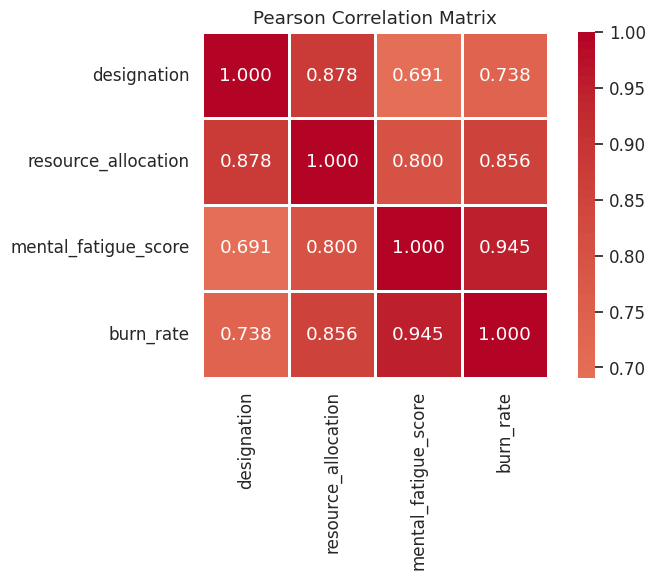
\includegraphics[width=0.75\linewidth]{10-correlation-heatmap.png}
  \caption{Pearson correlation heatmap of features and Burn Rate.}
  \label{fig:correlation-heatmap}
\end{figure}

\begin{figure}[H]
  \centering
  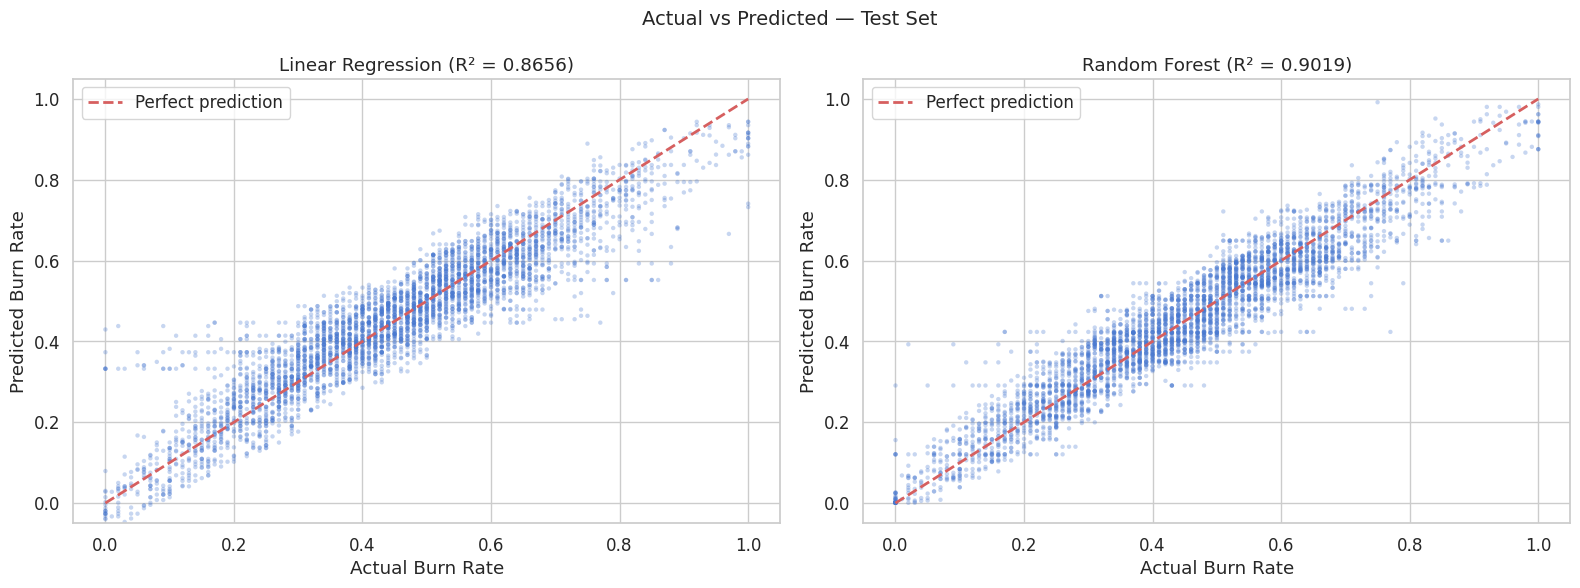
\includegraphics[width=0.90\linewidth]{11-actual-vs-predicted.png}
  \caption{Actual vs.\ predicted burn rate for both models.}
  \label{fig:actual-vs-predicted}
\end{figure}

\begin{figure}[H]
  \centering
  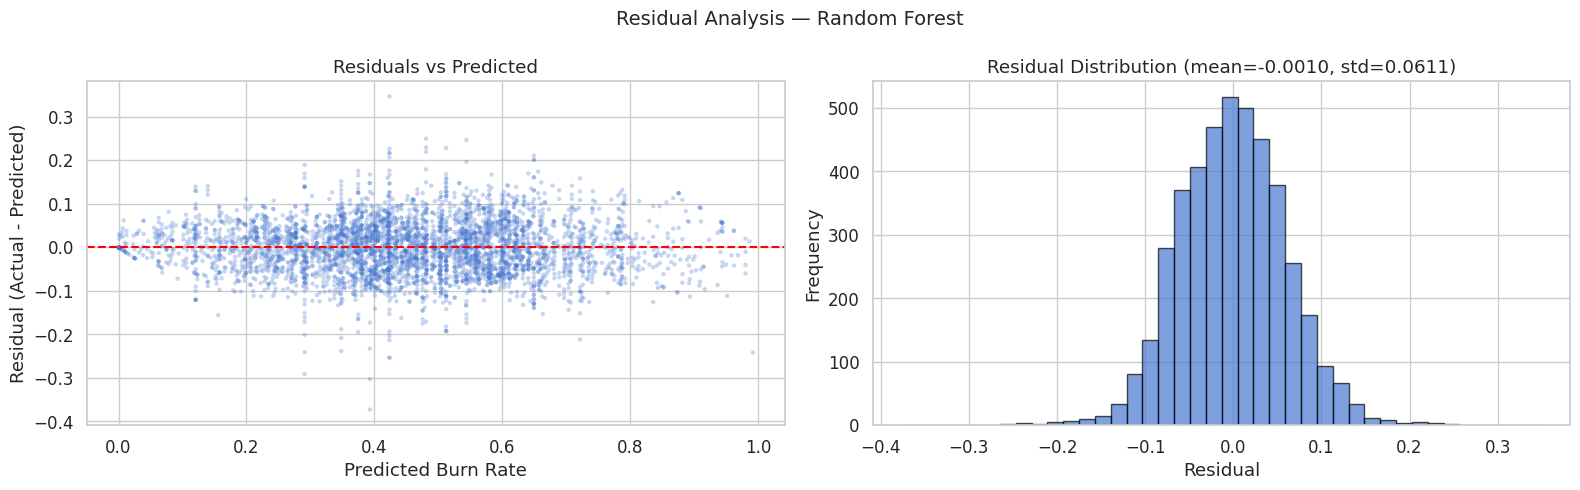
\includegraphics[width=0.90\linewidth]{12-residual-analysis.png}
  \caption{Residual analysis for the Random Forest model.}
  \label{fig:residual-analysis}
\end{figure}

\subsubsection{FastAPI Prediction Endpoint}

The prediction endpoint validates inputs using Pydantic models that enforce
strict ranges: designation (1--5), resource allocation (1--10), and mental
fatigue score (0--10). The model is loaded once at startup via a lifespan
handler and cached in memory. Each prediction call constructs a feature
array, runs \texttt{model.predict()}, clamps the result to the [0,~1]
range, and returns the burn rate in the standard envelope format. Response
times are consistently under 10~milliseconds.

\subsubsection{Integration with Express Backend}

The Express backend's \texttt{ai.service.js} implements a dual-mode
architecture controlled by the \texttt{AI\_USE\_MOCK} environment variable.
When set to \texttt{false}, the service sends an HTTP POST to the Python
endpoint with the three features and parses
\texttt{response.data.predictedBurnRate}. The request uses an
\texttt{AbortController} with a configurable timeout
(\texttt{AI\_SERVICE\_TIMEOUT\_MS}); timeouts and non-2xx responses are
wrapped as \texttt{ApiError.internal()} and surfaced to the frontend as a
generic 500 error.

When set to \texttt{true}, a mock formula is used in-process:
\begin{equation}
  \text{burnRate} = \text{clamp}_{[0,1]}\!\left(
    0.07 \cdot \text{mfs} + 0.03 \cdot d + 0.02 \cdot ra - 0.05
    + \text{noise}
  \right)
  \label{eq:mock-formula}
\end{equation}

\noindent where \textit{mfs} is the mental fatigue score, \textit{d} is
designation, \textit{ra} is resource allocation, and \textit{noise} is
uniform random in $[\!-0.025, +0.025]$. Switching between modes requires
no code changes---only an environment variable update and a server restart.

\subsection{Frontend Implementation}

\subsubsection{Authentication Pages}

The login and registration pages use a split-screen layout: the left panel
displays a brand illustration with a serif headline on a parchment
background, while the right panel contains the form on an ivory surface.
Forms are managed by react-hook-form with Zod validation schemas, ensuring
client-side validation before submission.

\begin{figure}[H]
  \centering
  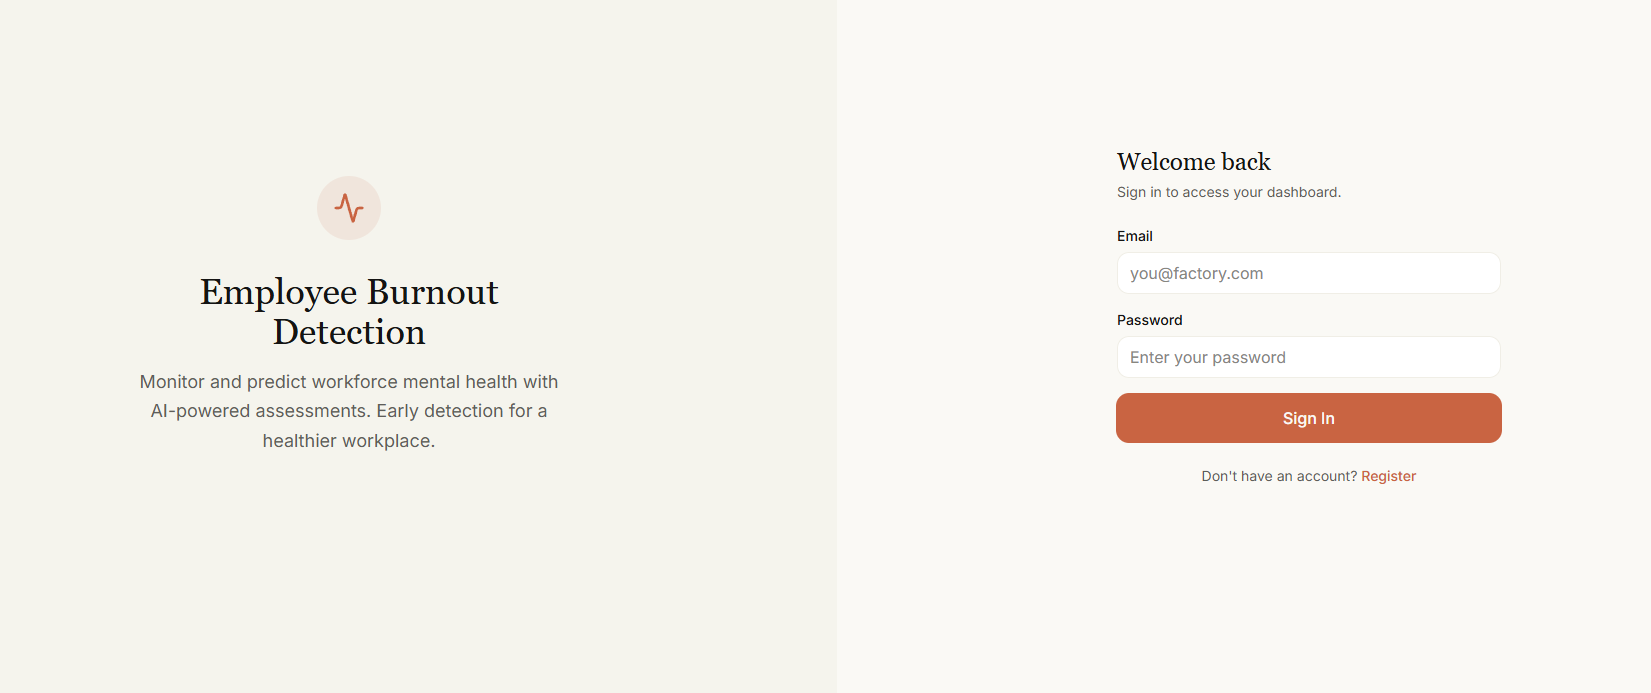
\includegraphics[width=0.95\linewidth]{13-screenshot-login.png}
  \caption{Login page with split-screen layout.}
  \label{fig:screenshot-login}
\end{figure}

\begin{figure}[H]
  \centering
  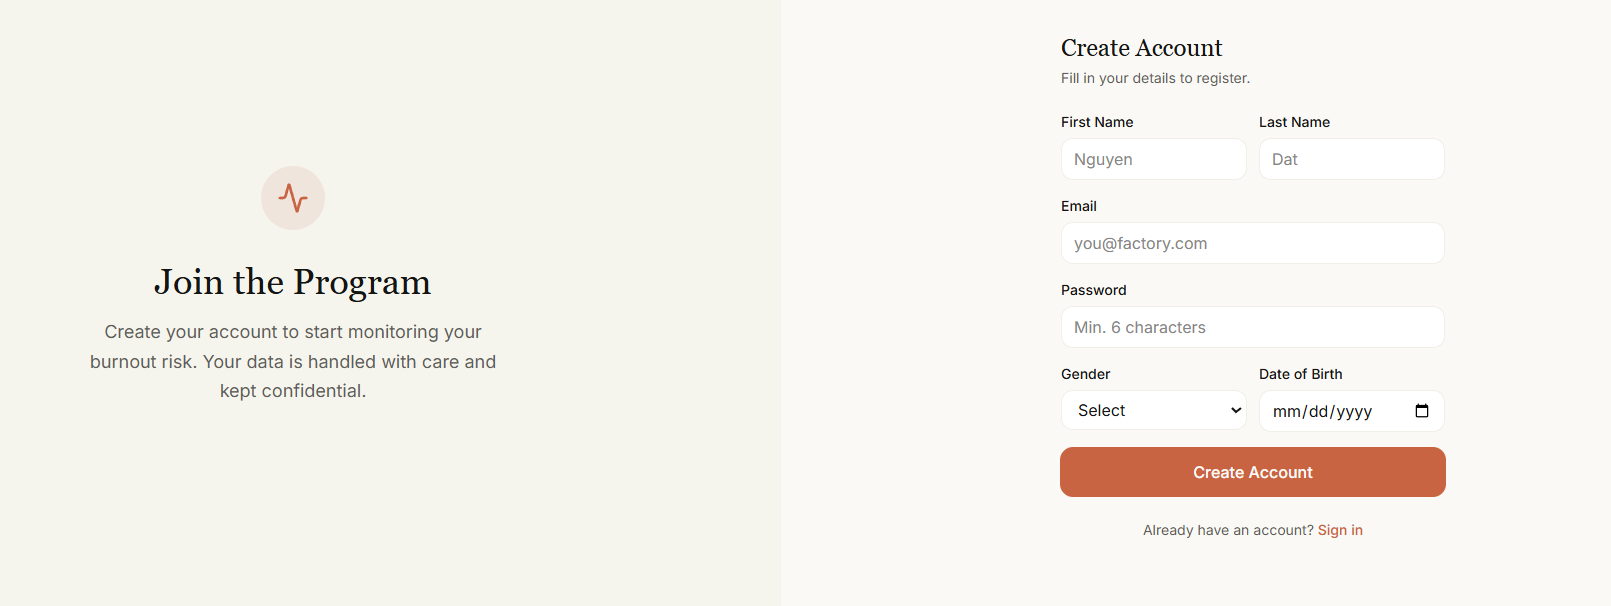
\includegraphics[width=0.95\linewidth]{14-screenshot-register.png}
  \caption{Registration page.}
  \label{fig:screenshot-register}
\end{figure}

\subsubsection{Employee Portal}

The employee portal consists of four pages accessible via a sidebar
navigation: Dashboard, Assessment, Results, and History.

\textbf{Employee Dashboard} (\texttt{/dashboard}). The central hub shows
the employee's profile information, a custom SVG semicircle burn rate
gauge with a needle indicator and colour-coded risk label, a bar chart
comparing personal vs.\ work-related burnout scores (0--100), and a line
chart plotting burn rate history over time with reference lines at the
0.35/0.55/0.80 risk thresholds. If the risk level is high or critical, a
``Get Help'' panel appears with curated mental health resources. If no
assessments exist, an empty state with a call-to-action to take the first
quiz is displayed.

\begin{figure}[H]
  \centering
  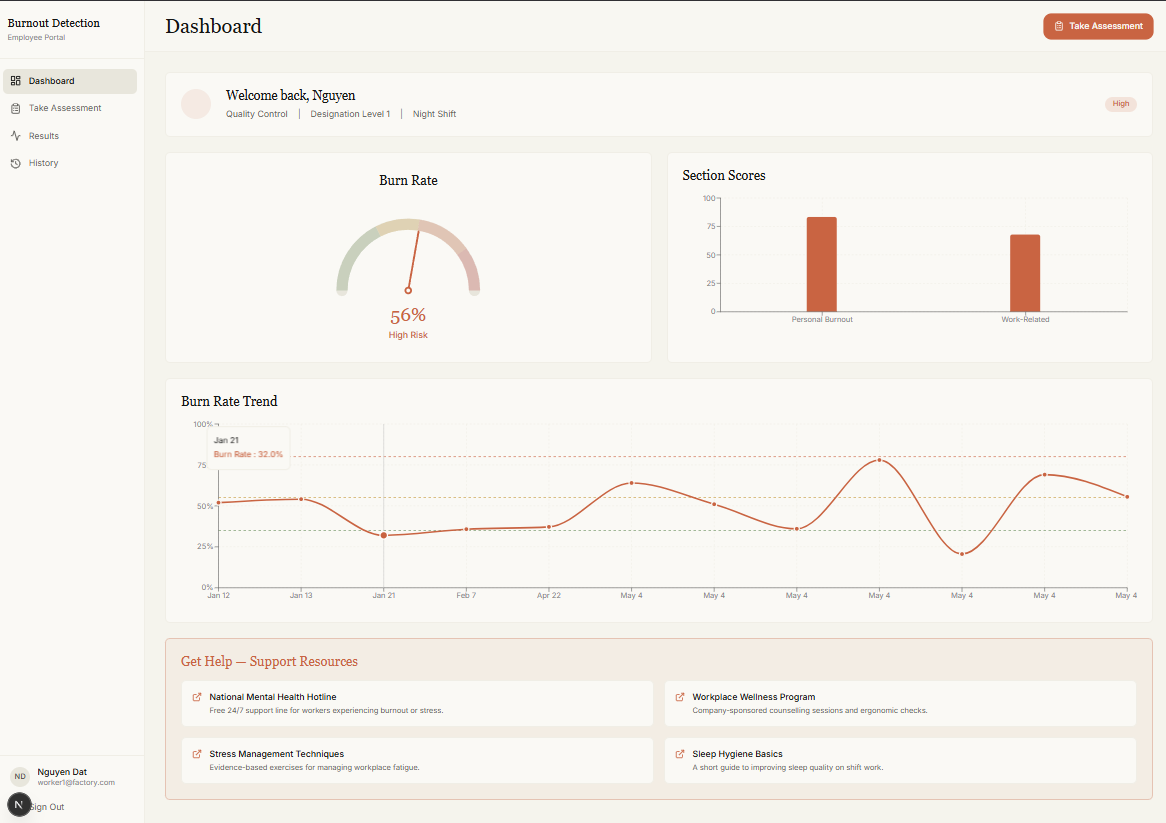
\includegraphics[width=0.95\linewidth]{15-screenshot-employee-dashboard.png}
  \caption{Employee dashboard with burn rate gauge and trend chart.}
  \label{fig:screenshot-employee-dashboard}
\end{figure}

\textbf{CBI Assessment} (\texttt{/assessment}). A two-step wizard
presents the 13 CBI questions. Step~1 covers Personal Burnout (questions
1--6) and Step~2 covers Work-Related Burnout (questions 7--13). Each
question displays five large clickable radio card options (Always, Often,
Sometimes, Seldom, Never/almost never). A progress bar shows the current
step. The ``Next'' button is disabled until all questions in the current
step are answered. On submission, the backend scores the quiz, calls the
AI service, and redirects the user to the results page.

\begin{figure}[H]
  \centering
  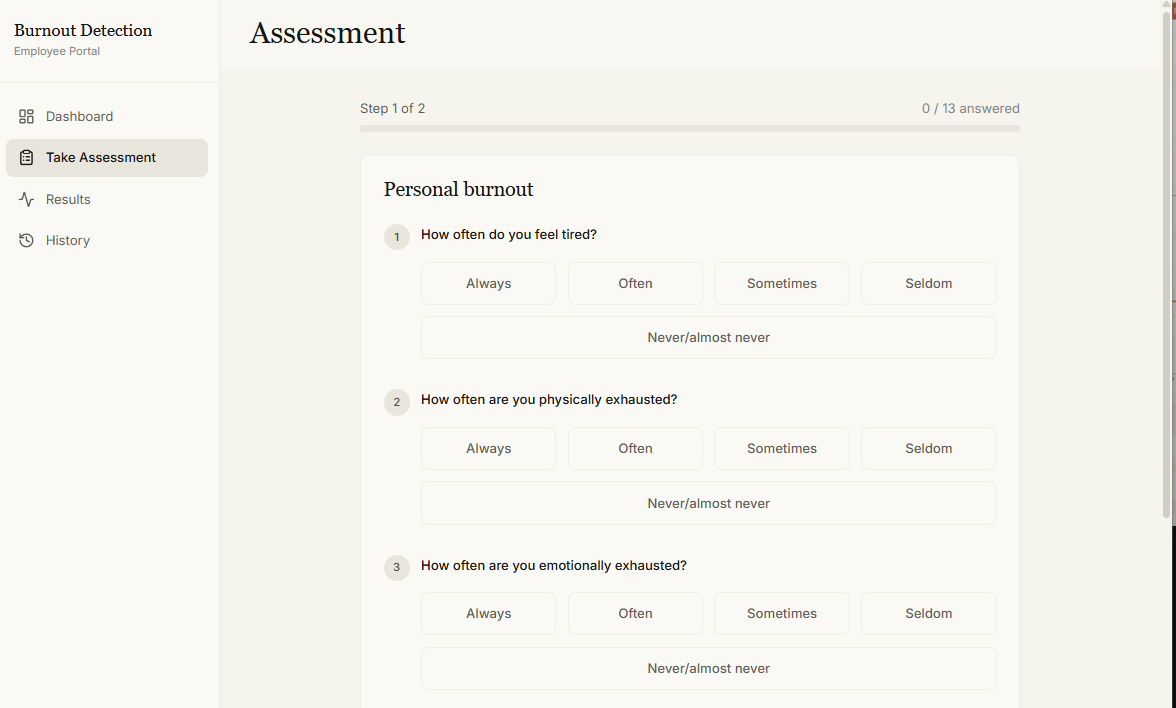
\includegraphics[width=0.95\linewidth]{16-screenshot-assessment.png}
  \caption{CBI assessment page --- Step 1: Personal Burnout.}
  \label{fig:screenshot-assessment}
\end{figure}

\textbf{Results} (\texttt{/results}). Displays the outcome of the most
recent assessment: a large burn rate gauge with risk-level badge, three
score cards (personal burnout, work-related burnout, mental fatigue), and
support resource cards filtered by the employee's current risk level.
Action buttons allow retaking the assessment or viewing history.

\begin{figure}[H]
  \centering
  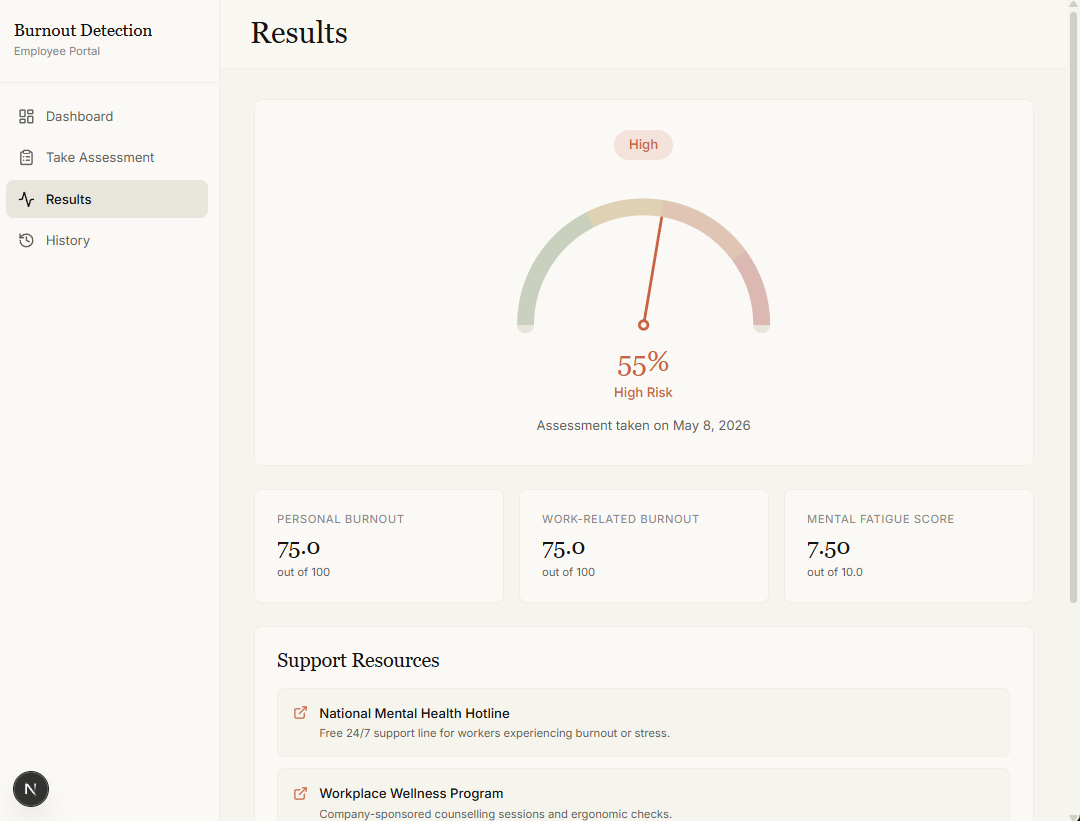
\includegraphics[width=0.95\linewidth]{17-screenshot-results.png}
  \caption{Assessment results page with score cards and support resources.}
  \label{fig:screenshot-results}
\end{figure}

\textbf{History} (\texttt{/history}). A paginated table listing all past
submissions with date, personal burnout average, work burnout average, and
quiz version. Each row is expandable to reveal the 13 individual responses
with labels and values; reverse-scored answers are annotated.

\begin{figure}[H]
  \centering
  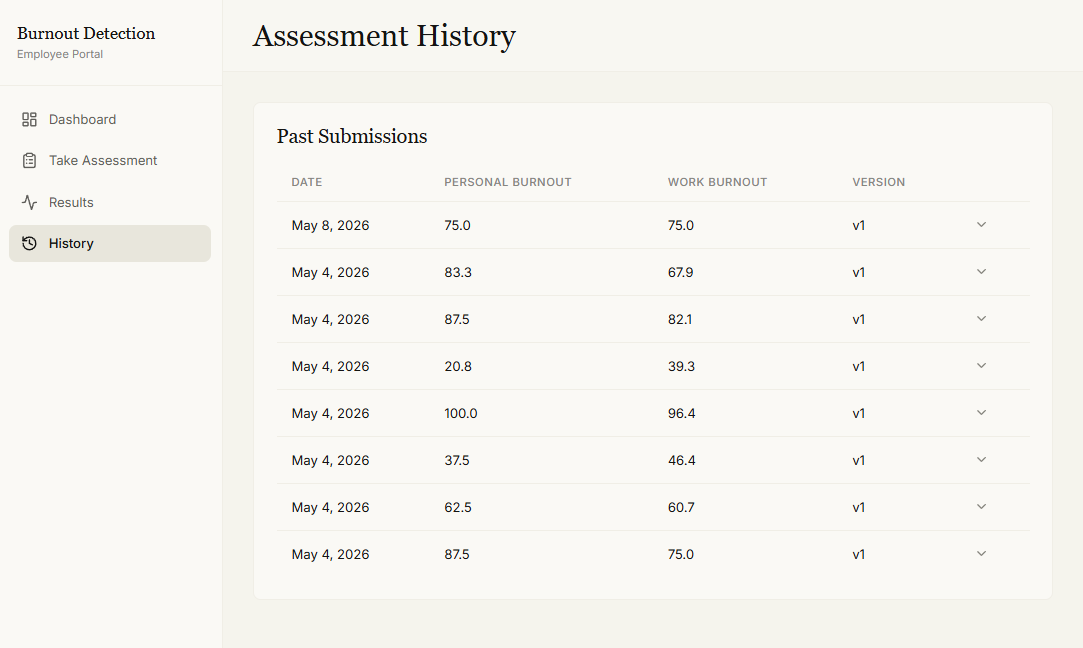
\includegraphics[width=0.95\linewidth]{18-screenshot-history.png}
  \caption{Quiz submission history with expandable response detail.}
  \label{fig:screenshot-history}
\end{figure}

\subsubsection{Admin Portal}

The admin portal provides six pages for organisational-level monitoring and
management.

\textbf{Admin Dashboard} (\texttt{/admin/dashboard}). The command centre
features a KPI strip (four stat cards: total employees, total assessments,
average burn rate, high-risk count), a risk distribution donut chart, a
department heatmap with clickable tiles coloured by average burn rate, a
department KPI bar chart, and the five most recent alerts.

\begin{figure}[H]
  \centering
  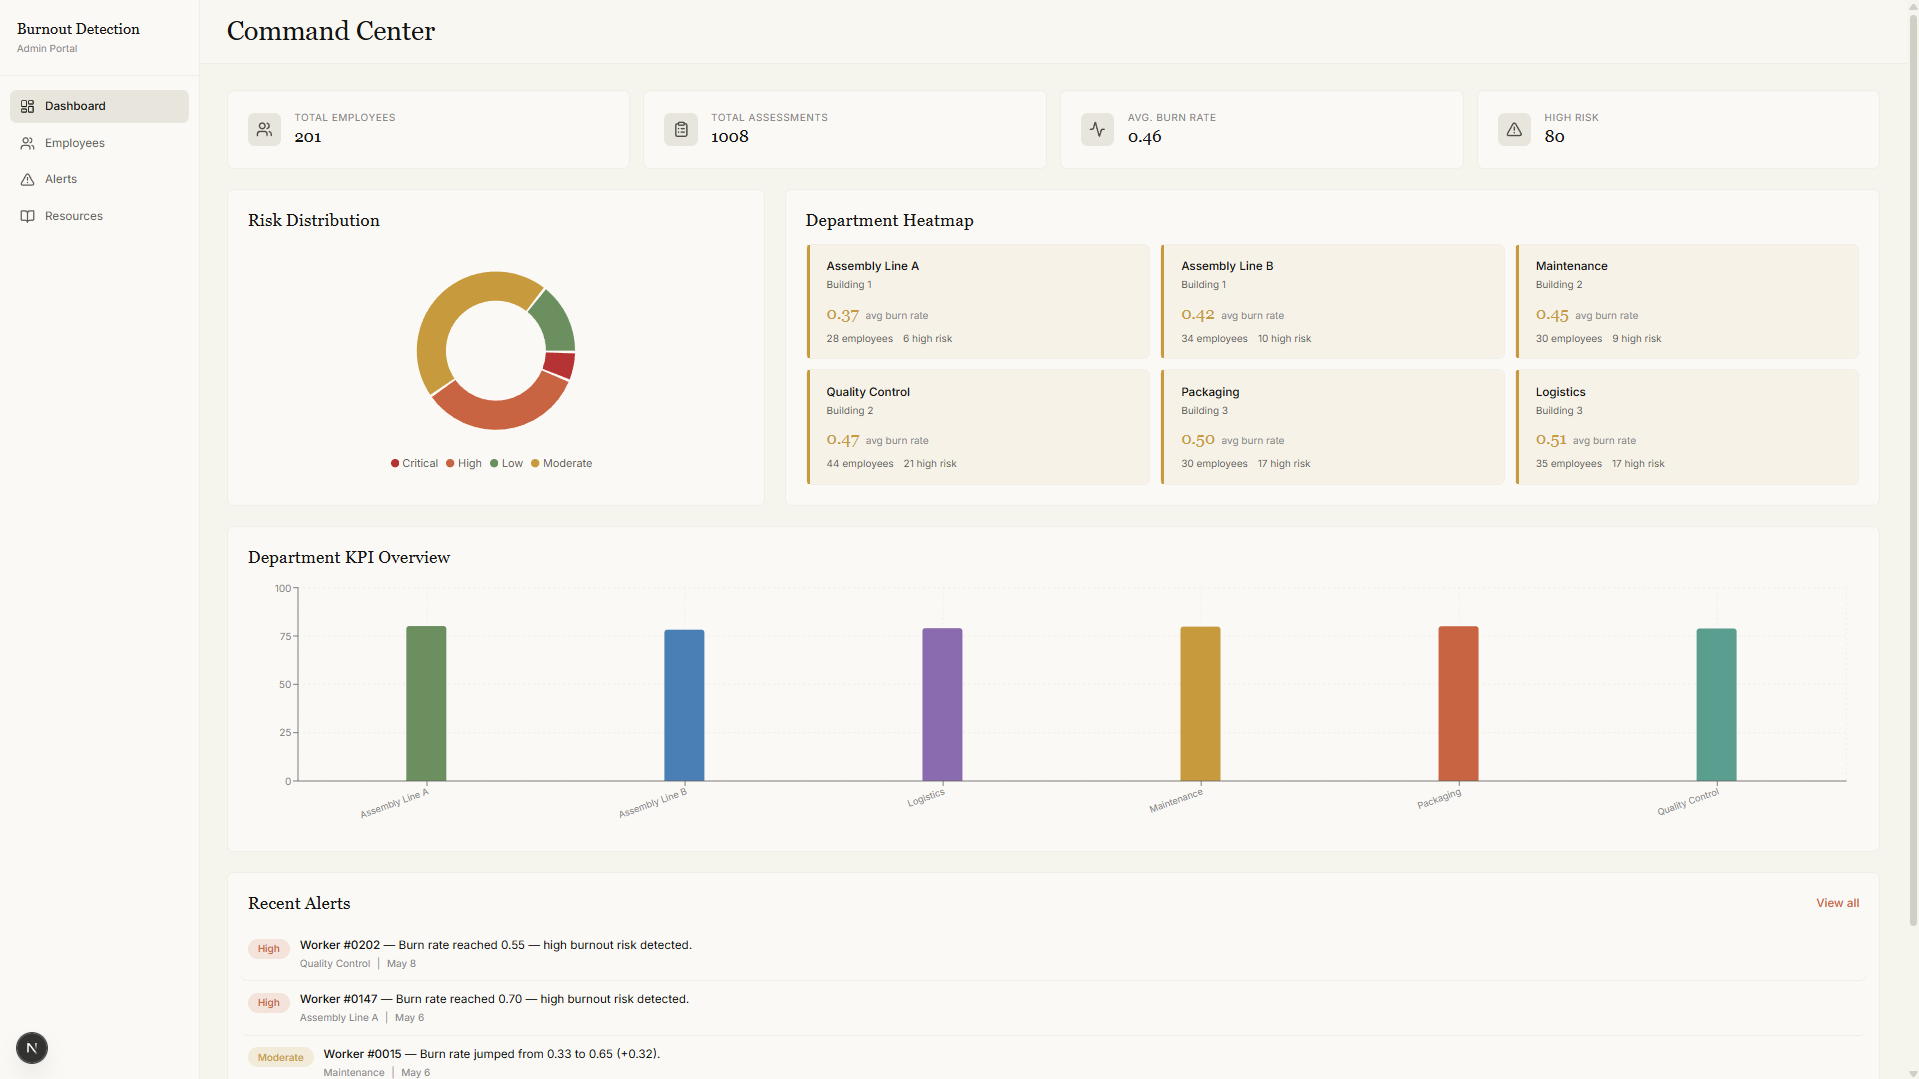
\includegraphics[width=0.95\linewidth]{19-screenshot-admin-dashboard.png}
  \caption{Admin command centre dashboard.}
  \label{fig:screenshot-admin-dashboard}
\end{figure}

\textbf{Department Detail} (\texttt{/admin/departments/[id]}). A two-tab
view: the \textit{Employees} tab shows a sortable, filterable, paginated
table of anonymised workers with risk badges, while the \textit{Analytics}
tab presents scatter plots, monthly burn rate trends, designation and shift
breakdowns, risk distribution, KPI trends, and KPI-vs-burn-rate
comparison charts.

\begin{figure}[H]
  \centering
  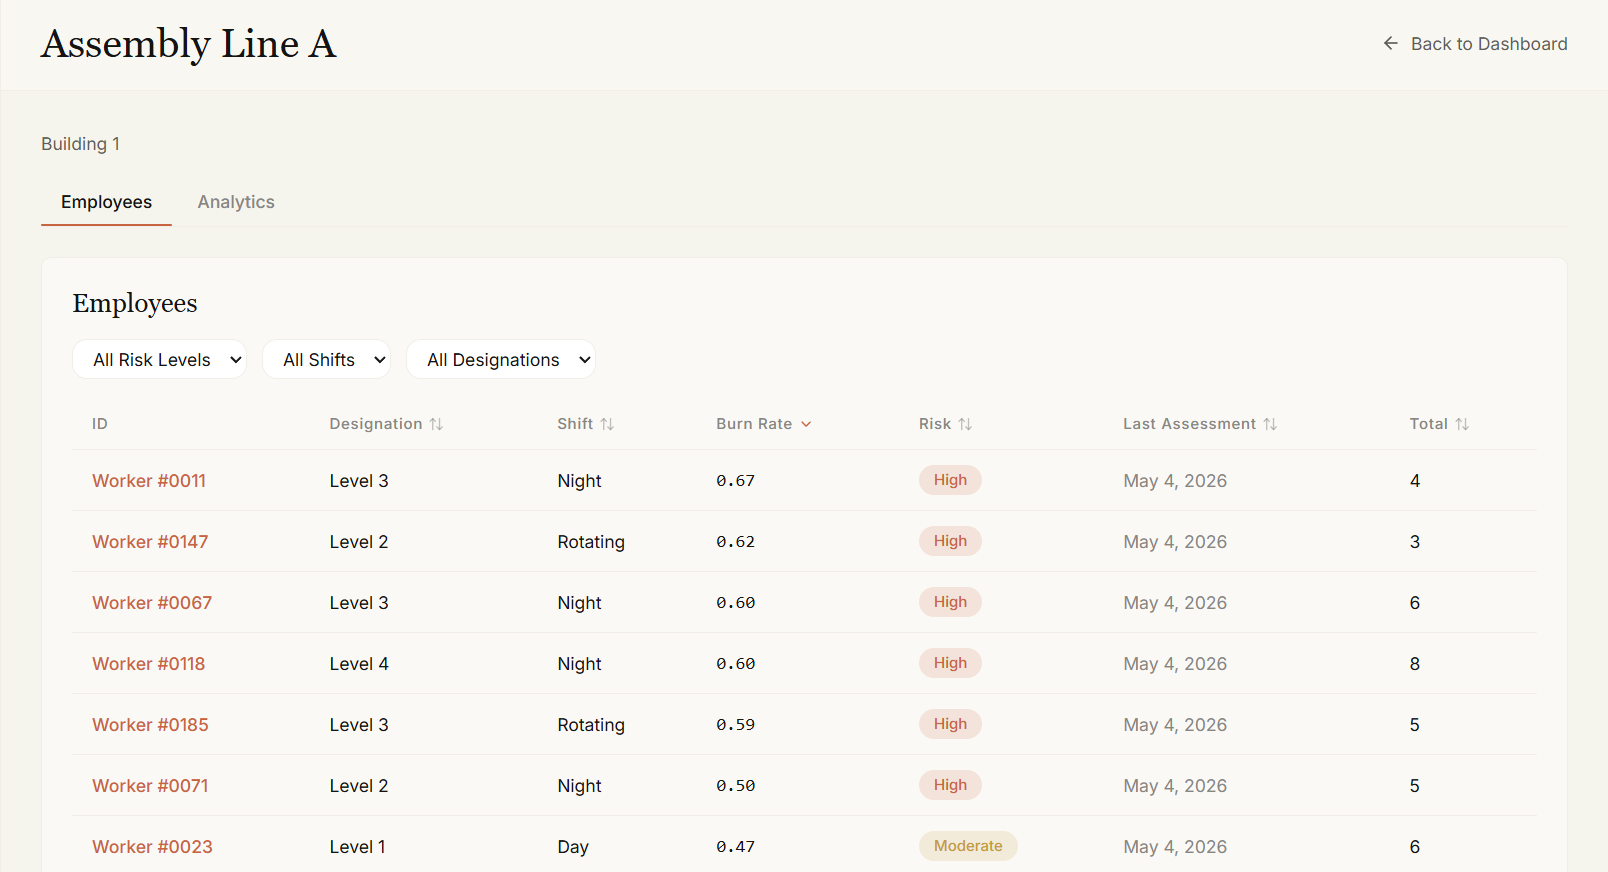
\includegraphics[width=0.95\linewidth]{20-screenshot-dept-employees.png}
  \caption{Department detail --- Employees tab with filters and sorting.}
  \label{fig:screenshot-dept-employees}
\end{figure}

\begin{figure}[H]
  \centering
  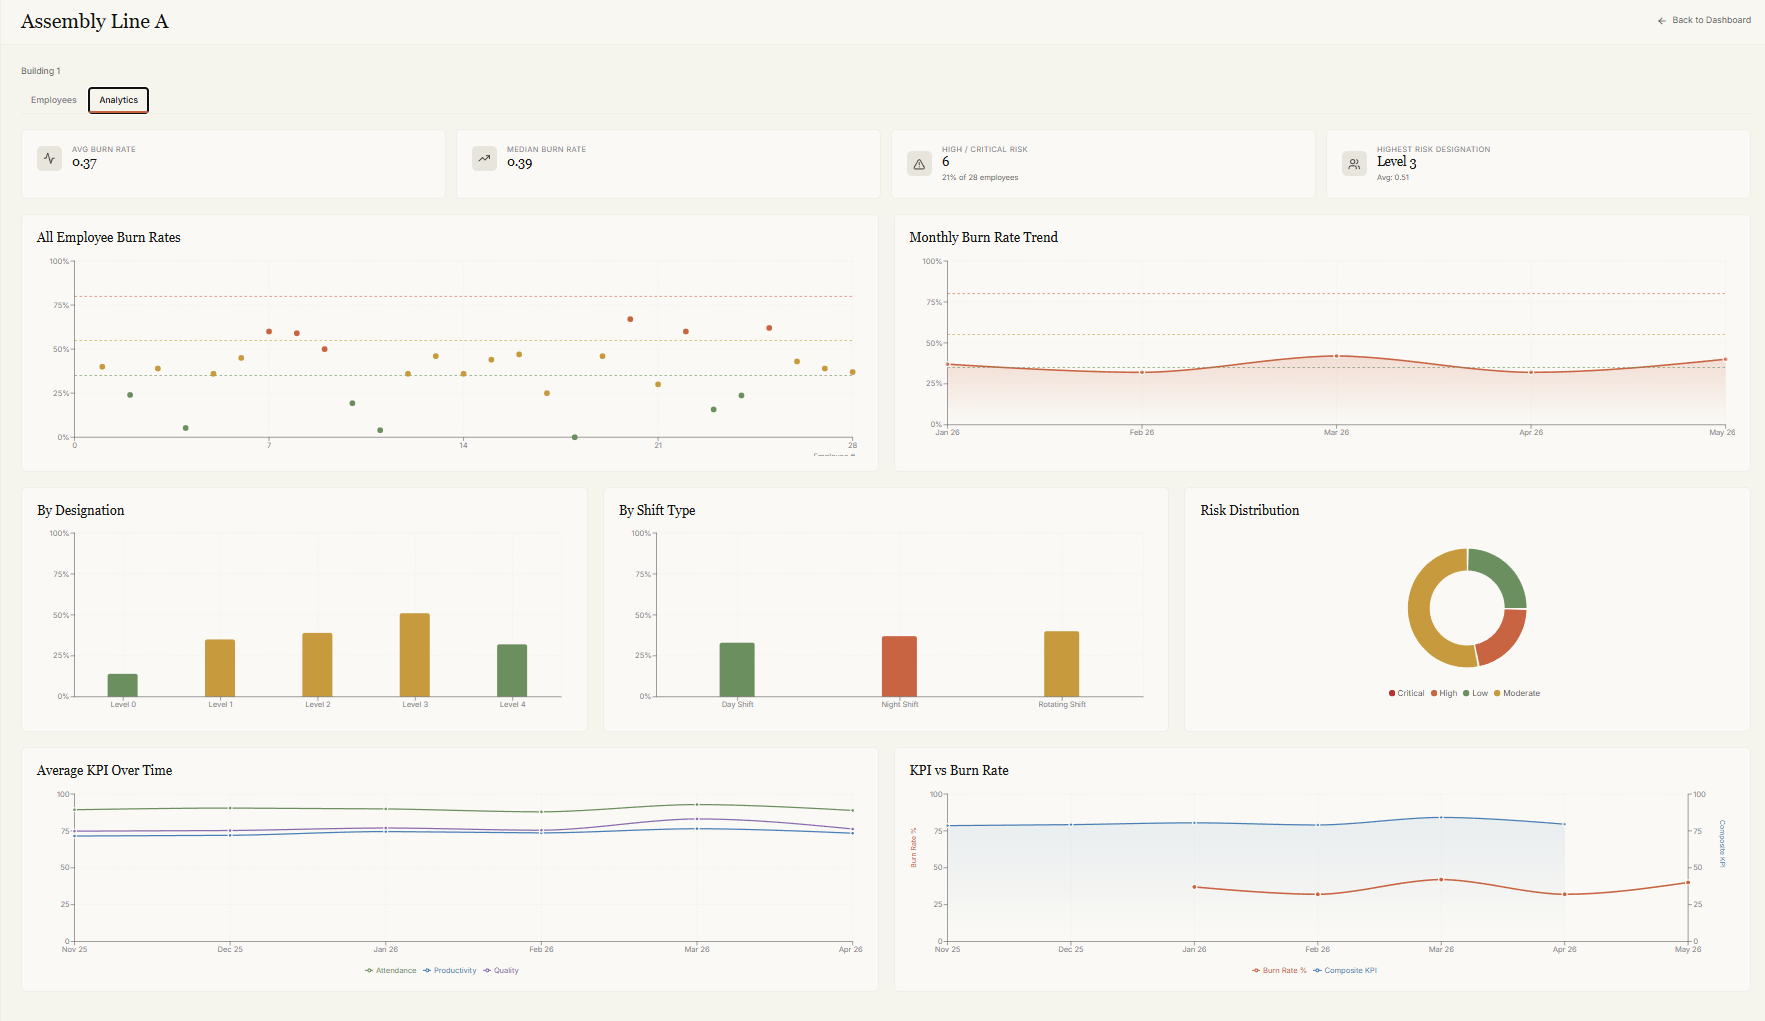
\includegraphics[width=0.95\linewidth]{21-screenshot-dept-analytics.png}
  \caption{Department detail --- Analytics tab with burnout and KPI visualisations.}
  \label{fig:screenshot-dept-analytics}
\end{figure}

\textbf{Employee Detail} (\texttt{/admin/employees/[id]}). A deep-dive
view for a single anonymised employee showing their burn rate gauge, burn
rate trend line chart, section score comparison, profile summary, monthly
KPI performance chart, and a dual-axis burn rate vs.\ KPI comparison chart.

\begin{figure}[H]
  \centering
  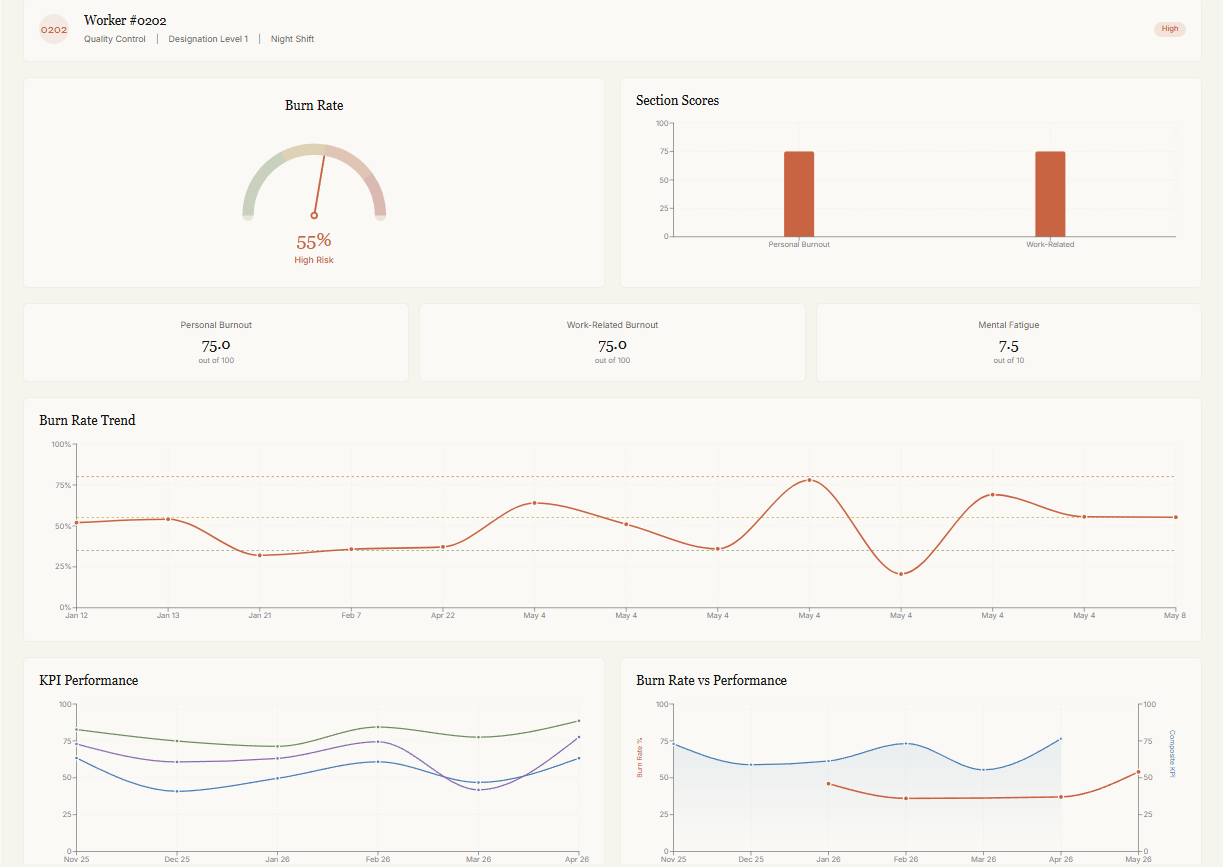
\includegraphics[width=0.95\linewidth]{22-screenshot-employee-detail.png}
  \caption{Admin employee detail with burnout and KPI analysis.}
  \label{fig:screenshot-employee-detail}
\end{figure}

\textbf{Alerts} (\texttt{/admin/alerts}). A filterable inbox with
dropdowns for read status and alert type, a table showing type badge,
department, message, date, and read status, and ``Mark read'' / ``Mark all
read'' actions. Mutations use TanStack Query cache invalidation for instant
UI updates.

\begin{figure}[H]
  \centering
  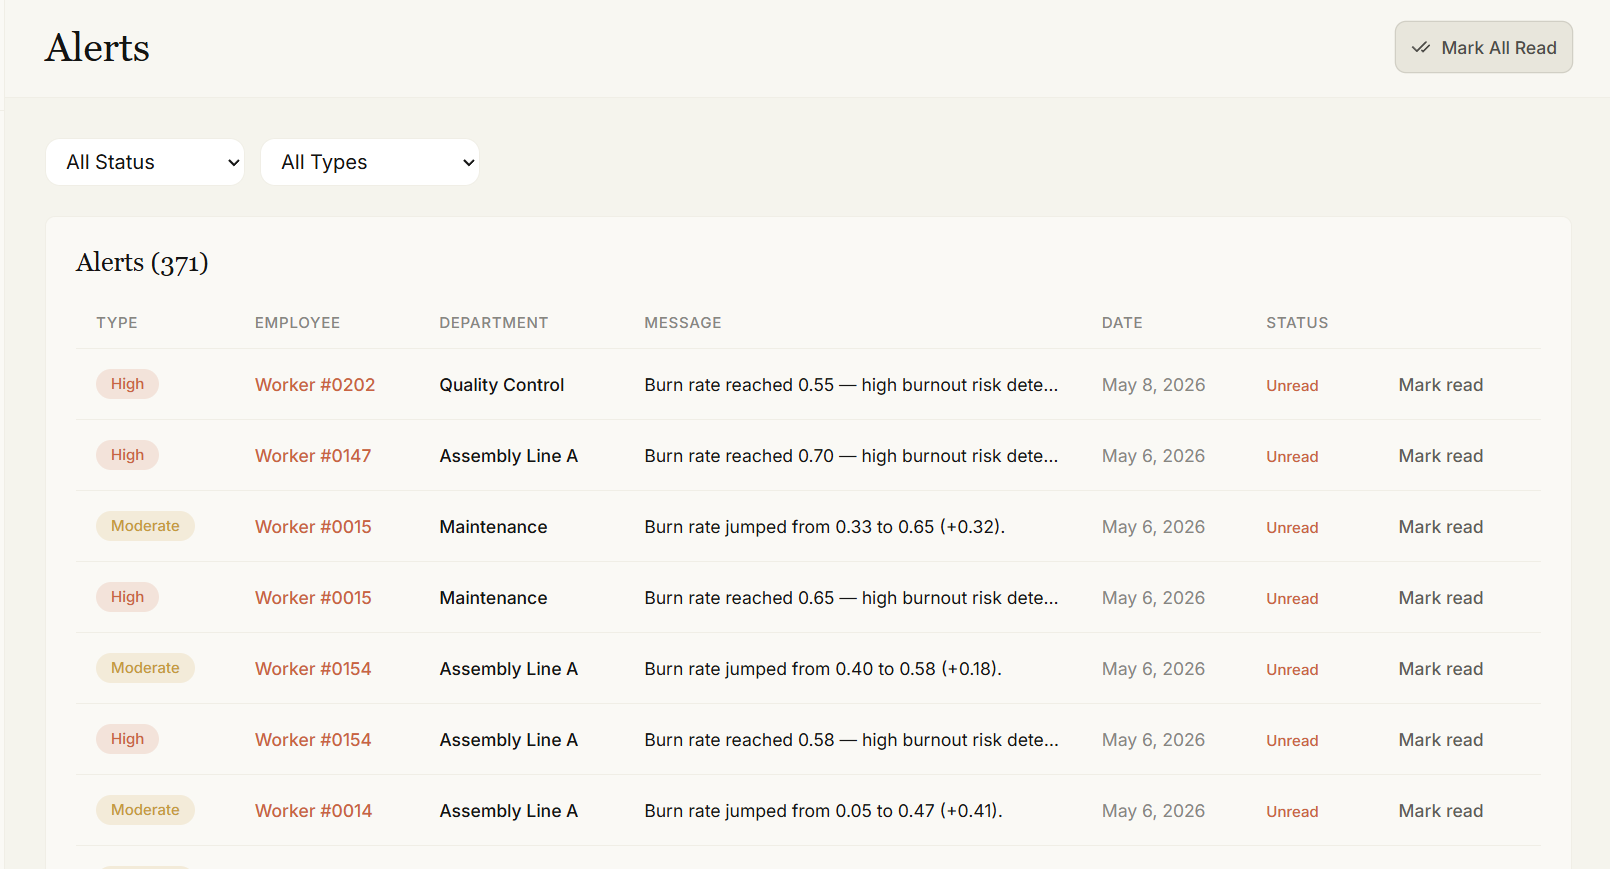
\includegraphics[width=0.95\linewidth]{23-screenshot-alerts.png}
  \caption{Admin alerts page with filtering.}
  \label{fig:screenshot-alerts}
\end{figure}

\textbf{Resource Management} (\texttt{/admin/resources}). Full CRUD for
help resources: a table lists all resources with title, description,
minimum risk level badge, active status, and URL. A modal form (validated
with Zod) handles creation and editing. Delete requires confirmation.
Toast notifications confirm successful operations.

\begin{figure}[H]
  \centering
  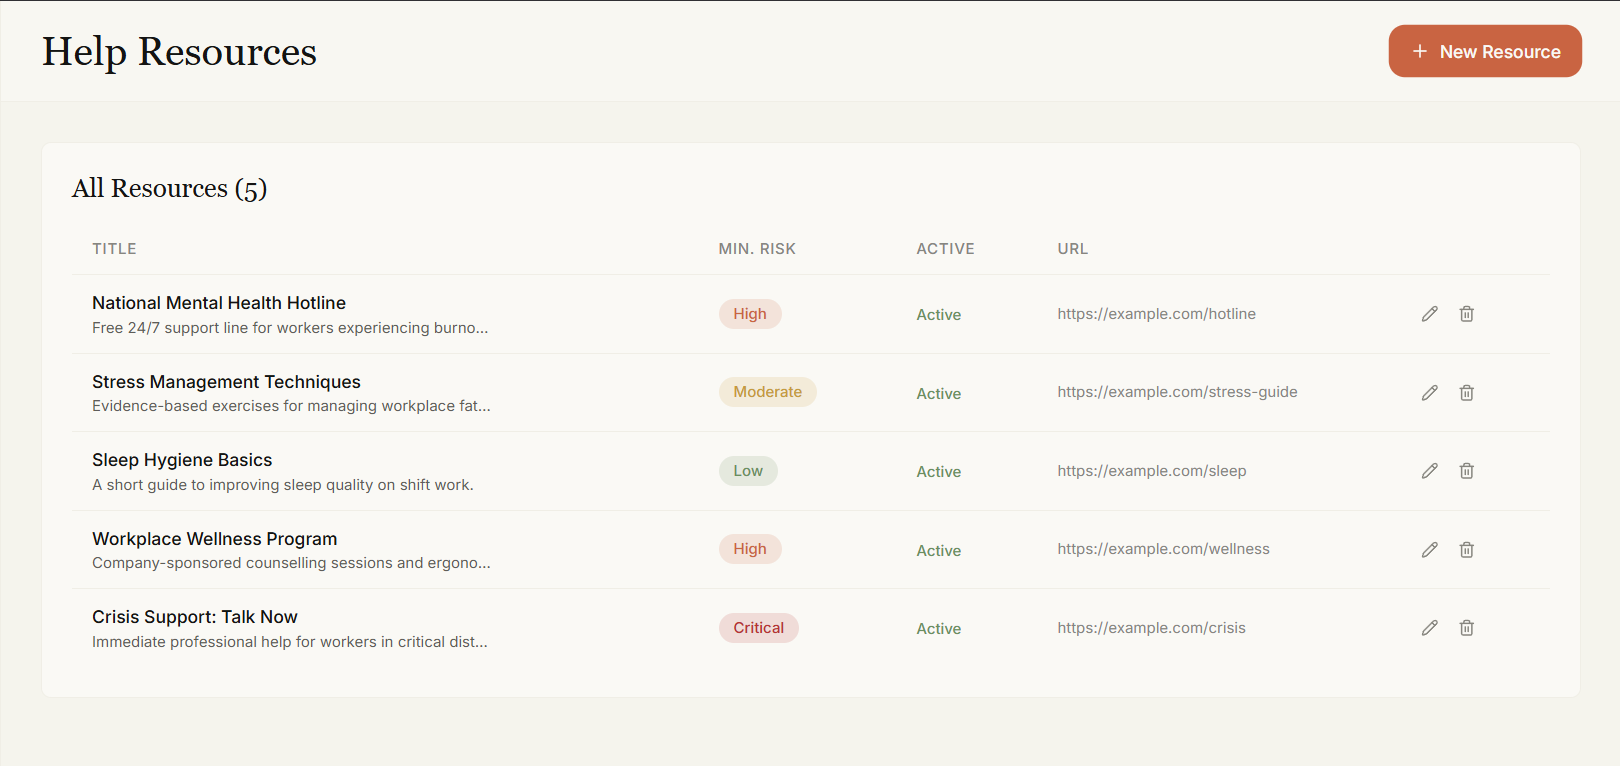
\includegraphics[width=0.95\linewidth]{24-screenshot-resources.png}
  \caption{Help resource management with CRUD operations.}
  \label{fig:screenshot-resources}
\end{figure}

\subsubsection{Reusable UI Components}

The frontend defines 15 reusable UI primitives in \texttt{components/ui/}
and 12 chart components in \texttt{components/charts/}. Notable custom
components include:

\begin{itemize}
  \item \textbf{BurnRateGauge:} A custom SVG semicircle gauge that renders
    a colour-gradient arc from green through amber to red, with an animated
    needle positioned at the current burn rate value and a risk-level label
    beneath.

  \item \textbf{DepartmentHeatmap:} A tile grid where each department is
    rendered as a clickable card with its name, employee count, and
    background colour interpolated from the risk colour scale based on the
    department's average burn rate.

  \item \textbf{KpiBurnRateComparisonChart:} A Recharts composed chart
    with dual Y-axes, plotting composite KPI (bar) against average burn
    rate (line) over monthly periods to reveal inverse correlations.
\end{itemize}

\subsubsection{State Management with TanStack Query}

All server state is managed through TanStack Query (React Query), which
provides automatic caching, background refetching, and cache invalidation.
Custom hooks in \texttt{lib/hooks/} wrap \texttt{useQuery} for read
operations and \texttt{useMutation} for write operations. Mutations
automatically invalidate related query keys on success, ensuring the UI
stays synchronised with the server without manual refetch calls.

Loading states are handled with skeleton placeholders (pulsing sand-coloured
blocks), error states display inline messages in crimson-tinted cards, and
empty data sets show an \texttt{EmptyState} component with an icon,
descriptive text, and a call-to-action button.



\clearpage
\section{Discussion and Evaluation}

\subsection{Model Performance Analysis}

The Random Forest model achieves an $R^{2}$ of 0.90, an MAE of 0.048, and
an RMSE of 0.061 on the held-out test set
(Table~\ref{tab:model-comparison}). These results indicate that the model
explains 90\% of the variance in burn rate and is typically accurate to
within 5 percentage points on the 0--1 scale. The 3.6 percentage-point
improvement in $R^{2}$ over Linear Regression demonstrates that the
Random Forest captures meaningful non-linear interactions between the three
features---interactions that a linear model cannot represent without manual
feature engineering.

Feature importance analysis reveals that mental fatigue score accounts for
approximately 85\% of the model's predictive power, with resource
allocation contributing around 10\% and designation approximately 5\%.
This distribution is consistent with domain knowledge: an employee's
psychological state is the most direct indicator of burnout risk, while
workload intensity and seniority play secondary roles. The strong
dominance of mental fatigue score also validates the system's architecture,
which places the CBI quiz---the source of the mental fatigue score---at
the centre of the assessment workflow.

The residual analysis (Figure~\ref{fig:residual-analysis}) shows that
prediction errors are approximately randomly distributed around zero with
no systematic pattern, indicating that the model does not exhibit
consistent over- or under-prediction across the burn rate range. The
residual distribution is approximately normal, centred at zero, which is a
desirable property for a regression model.

Compared to public Kaggle notebooks that train on the same dataset with
all available features, the system's $R^{2}$ of 0.90 using only three
features falls within the reported range of 0.90--0.93 for Random Forest
models. This suggests that the three selected features capture the
majority of the predictive signal, and the additional columns (Gender,
Company Type, WFH Setup) contribute relatively little to burn rate
prediction.

\subsection{Functional Testing}

The system was tested end-to-end through manual testing of all user flows.
Table~\ref{tab:test-cases} summarises the key test cases and their
outcomes.

\begin{longtable}{@{}p{0.40\linewidth}p{0.35\linewidth}c@{}}
  \caption{Functional test cases and results.}
  \label{tab:test-cases} \\
  \toprule
  \textbf{Test Case} & \textbf{Expected Behaviour} & \textbf{Result} \\
  \midrule
  \endfirsthead
  \toprule
  \textbf{Test Case} & \textbf{Expected Behaviour} & \textbf{Result} \\
  \midrule
  \endhead
  \bottomrule
  \endfoot

  Employee registration with valid data
    & User created, HR profile generated, JWT returned
    & Pass \\
  Registration with duplicate email
    & 409 Conflict error returned
    & Pass \\
  Login with valid credentials
    & JWT issued, redirect to dashboard
    & Pass \\
  Login with wrong password
    & 401 Unauthorized error
    & Pass \\
  Fetch CBI quiz questions
    & 13 questions with sections and options returned
    & Pass \\
  Submit quiz with all 13 answers
    & Scores calculated, AI called, result saved
    & Pass \\
  Submit quiz with missing answers
    & 400 Validation error
    & Pass \\
  Reverse scoring (question 10)
    & adjustedValue = 100 $-$ rawValue
    & Pass \\
  Mental fatigue score calculation
    & Correct value per Equation~\ref{eq:fatigue}
    & Pass \\
  AI prediction returns valid burn rate
    & Value in [0, 1] range
    & Pass \\
  Risk level mapping
    & Correct threshold applied
    & Pass \\
  Alert generated on high risk
    & \texttt{high\_risk} alert created
    & Pass \\
  Alert generated on trend spike
    & \texttt{trend\_spike} alert (delta $\geq$ 0.15)
    & Pass \\
  Employee dashboard data
    & Profile, gauge, trend, section scores
    & Pass \\
  Admin dashboard aggregation
    & Dept.\ stats, risk distribution, KPIs
    & Pass \\
  Department drill-down with filters
    & Correct filtering and sorting
    & Pass \\
  Department analytics charts
    & All chart data populated
    & Pass \\
  Employee detail (admin view)
    & KPI and burn rate data displayed
    & Pass \\
  Mark alert as read
    & Alert status updated, cache invalidated
    & Pass \\
  Resource CRUD (create, update, delete)
    & Resource persisted, table refreshed
    & Pass \\
  Route guard (employee accessing admin)
    & Redirect to employee dashboard
    & Pass \\
  Route guard (unauthenticated access)
    & Redirect to login page
    & Pass \\
  JWT expiry handling
    & 401 response, redirect to login
    & Pass \\
\end{longtable}

All 23 test cases passed, confirming that the core workflows function as
designed. Testing covered authentication, quiz scoring, AI integration,
dashboard aggregation, alert generation, CRUD operations, and access
control.

\subsection{System Feature Evaluation}

Table~\ref{tab:objective-eval} evaluates each objective defined in
Section~1.4 against the implemented system features.

\begin{longtable}{@{}cp{0.45\linewidth}p{0.30\linewidth}@{}}
  \caption{Evaluation of system objectives.}
  \label{tab:objective-eval} \\
  \toprule
  \textbf{Obj.} & \textbf{Description} & \textbf{Status} \\
  \midrule
  \endfirsthead
  \toprule
  \textbf{Obj.} & \textbf{Description} & \textbf{Status} \\
  \midrule
  \endhead
  \bottomrule
  \endfoot

  1 & Implement CBI-based assessment with mental fatigue scoring
    & Fully implemented \\
  2 & Train ML model for burn rate prediction
    & Achieved ($R^{2} = 0.90$) \\
  3 & Build employee self-monitoring portal
    & Fully implemented (4 pages) \\
  4 & Build admin command centre with analytics
    & Fully implemented (6 pages) \\
  5 & Implement automated risk alerting
    & Fully implemented (3 alert types) \\
  6 & Demonstrate microservice architecture
    & Fully implemented (3 services) \\
\end{longtable}

All six objectives have been achieved. The employee portal provides
comprehensive self-monitoring with gauge visualisations, trend charts, and
support resources. The admin portal offers department-level heatmaps, risk
distribution analytics, KPI correlation views, and a fully functional
alert inbox. The microservice architecture cleanly separates the ML concern
from the web backend.

\subsection{Answering the Research Questions}

\textbf{RQ1: How effectively can a Random Forest regression model predict
employee burn rate using only three input features?}

The Random Forest model achieves an $R^{2}$ of 0.90 with an MAE of 0.048,
demonstrating that three features---designation, resource allocation, and
mental fatigue score---are sufficient for effective burn rate prediction.
The model's performance is comparable to published results that use the
full feature set, indicating that the three selected features capture the
dominant signal in the data.

\textbf{RQ2: Can a web-based system provide actionable burnout insights to
both employees and HR administrators?}

The employee portal provides personalised burn rate gauges, historical
trend charts, section score breakdowns, and contextual help resources,
enabling workers to monitor their own mental health proactively. The admin
portal provides department heatmaps, risk distribution charts,
KPI-vs-burn-rate correlations, and automated alerts, giving HR managers
actionable visibility into organisational burnout patterns. The functional
testing results confirm that all data flows correctly from quiz submission
through prediction to dashboard visualisation.

\textbf{RQ3: What are the practical benefits and trade-offs of using a
microservice architecture to separate ML inference from the application
backend?}

The microservice architecture provides three concrete benefits:
(1)~technology heterogeneity---Python's scikit-learn ecosystem for ML and
JavaScript's Express ecosystem for web logic are each used where they excel;
(2)~independent development---the AI service can be retrained and redeployed
without modifying or restarting the backend; (3)~the mock/real switch
(\texttt{AI\_USE\_MOCK}) enables fully functional development without running
the Python service. The primary trade-off is increased operational
complexity: two servers must be running and communicating, and network
failures between them require timeout handling and error propagation.

\subsection{Comparison with Related Work}

As summarised in Table~\ref{tab:related-comparison}, this system is the
only solution among the reviewed works that combines all four elements: a
trained ML model, a deployed web application, organisational-level
analytics, and a validated burnout instrument (CBI).

Pradhan and Jena's framework~\cite{pradhan2019} uses machine learning for
burnout classification but lacks a web deployment and does not provide
organisational dashboards. Commercial platforms like Culture
Amp~\cite{cultureamp2024} offer web-based analytics but rely on
general-purpose engagement surveys without ML prediction. Kaggle community
notebooks~\cite{kaggle2021} demonstrate model training on the same dataset
but do not integrate predictions into a usable application.

This thesis fills the integration gap by unifying psychometric assessment,
machine learning prediction, and multi-level analytics into a single
platform that serves both individual workers and organisational decision
makers.




\clearpage
\section{Conclusion and Future Work}

\subsection{Conclusion}

This thesis presented the design, implementation, and evaluation of an
intelligent web-based framework for the early detection of employee burnout
in industrial workplaces. The system integrates a validated psychometric
instrument (the Copenhagen Burnout Inventory), a machine learning
prediction model (Random Forest regression), and a full-stack web
application with role-based portals for both employees and administrators.

The Random Forest model, trained on approximately 22{,}000 records from a
public dataset, achieves an $R^{2}$ of 0.90 using only three input
features, demonstrating that effective burn rate prediction is possible
from a minimal feature set. The employee portal empowers workers with
self-monitoring tools---burn rate gauges, trend charts, and contextual
support resources---while the admin portal provides organisational-level
visibility through department heatmaps, risk distribution analytics, KPI
correlations, and automated alerts.

The microservice architecture successfully separates the machine learning
concern (Python/FastAPI) from the web application backend
(Node.js/Express), enabling independent development and deployment.
End-to-end functional testing confirmed that all core workflows operate
correctly, from quiz submission and scoring through AI prediction to
dashboard visualisation and alert generation.

\subsection{Contributions}

This thesis makes the following contributions:

\begin{enumerate}
  \item \textbf{An integrated burnout detection platform} that combines
    psychometric assessment, machine learning prediction, and
    multi-level organisational analytics within a single web-based
    system---a combination not found in any of the reviewed related
    works.

  \item \textbf{A practical CBI-to-ML pipeline} that transforms
    13-question Copenhagen Burnout Inventory responses into a continuous
    burn rate prediction through a clearly documented scoring and
    feature engineering process, including reverse scoring, section
    averaging, and normalisation.

  \item \textbf{A demonstrable microservice pattern} for integrating
    machine learning into web applications, with a clean
    mock/real switch mechanism that enables independent development of
    the ML and web components.

  \item \textbf{A comprehensive admin analytics suite} including
    department heatmaps, risk distribution charts, KPI-vs-burn-rate
    correlations, and automated three-type alert generation
    (high risk, critical risk, and trend spike).

  \item \textbf{A complete design system and component library} with
    15 reusable UI primitives and 12 data visualisation components,
    including a custom SVG burn rate gauge.
\end{enumerate}

\subsection{Achievement of Objectives}

All six objectives defined in Section~1.4 have been fully achieved:

\begin{enumerate}
  \item The CBI-based assessment is implemented as a two-step wizard with
    proper reverse scoring and mental fatigue score derivation.

  \item The Random Forest model achieves $R^{2} = 0.90$, MAE = 0.048,
    and RMSE = 0.061, significantly outperforming the Linear Regression
    baseline.

  \item The employee portal includes four fully functional pages:
    dashboard, assessment, results, and history.

  \item The admin portal includes six pages: command centre, department
    detail (with employees and analytics tabs), company-wide employee
    list, individual employee detail, alerts inbox, and resource
    management.

  \item Three alert types (high risk, critical risk, and trend spike) are
    automatically generated and displayed in a filterable inbox with
    mark-read functionality.

  \item The three-service architecture (React/Next.js, Node.js/Express,
    Python/FastAPI) is fully operational with mock/real mode switching.
\end{enumerate}

\subsection{Limitations}
\label{sec:limitations}

Several limitations should be acknowledged:

\begin{itemize}
  \item \textbf{Simulated HR data.} Designation and resource allocation
    values are randomly generated at registration rather than sourced
    from a real factory HR system. While values are drawn from the
    training dataset's ranges, they do not reflect actual workplace
    conditions.

  \item \textbf{Limited feature set.} The model uses only three
    features. Including additional signals such as actual shift
    patterns, overtime records, or longitudinal CBI trends could improve
    predictive accuracy.

  \item \textbf{Single dataset.} Model training and evaluation rely on a
    single public Kaggle dataset. The model's performance may not
    generalise across different industries, cultures, or organisational
    contexts.

  \item \textbf{Simulated KPI data.} The employee KPI records
    (attendance, productivity, quality) are seeded rather than collected
    from real workplace systems, limiting the validity of the
    KPI-vs-burn-rate correlation analysis.

  \item \textbf{Desktop-only interface.} The application is designed for
    minimum 992~px screen widths. Factory workers using personal mobile
    devices cannot access the system.

  \item \textbf{No formal usability study.} The system was tested
    functionally but not evaluated through a structured usability study
    with real end users.

  \item \textbf{No real-time updates.} The admin dashboard uses
    polling-based data fetching via TanStack Query rather than real-time
    push notifications via WebSocket or Server-Sent Events.
\end{itemize}

\subsection{Future Work}
\label{subsec:future}

The following directions are proposed for future development:

\begin{itemize}
  \item \textbf{Mobile responsive design.} Extend the frontend with
    responsive breakpoints to support mobile and tablet access, enabling
    factory workers to complete assessments on personal devices.

  \item \textbf{Real-time alerts.} Implement WebSocket or Server-Sent
    Events to push new alerts to the admin dashboard instantly, without
    requiring page refresh or polling intervals.

  \item \textbf{Integration with real HR systems.} Replace the simulated
    HR profile generator with connectors to actual HR information
    systems (e.g., SAP SuccessFactors, BambooHR) to provide authentic
    designation and workload data.

  \item \textbf{Advanced ML models.} Explore Gradient Boosting
    (XGBoost, LightGBM) and time-series models that incorporate
    longitudinal CBI trends, enabling the system to predict burn rate
    trajectories rather than point estimates.

  \item \textbf{Expanded feature engineering.} Incorporate additional
    features such as actual overtime hours, shift rotation frequency,
    and seasonal patterns to improve model accuracy.

  \item \textbf{Export functionality.} Add CSV and PDF export for
    department analytics reports and assessment history, enabling
    offline review and reporting.

  \item \textbf{Accessibility improvements.} Add ARIA labels to custom
    components (gauge, heatmap) and conduct automated accessibility
    testing to ensure compliance with WCAG guidelines.

  \item \textbf{Multi-language support.} Internationalise the user
    interface to support Vietnamese and other languages relevant to the
    target industrial workforce.

  \item \textbf{Formal usability evaluation.} Conduct a structured
    usability study with factory workers and HR personnel to validate
    the system's effectiveness and identify user experience
    improvements.
\end{itemize}



% ════════════════════════════════════════════════════════════════════════════
%  REFERENCES
% ════════════════════════════════════════════════════════════════════════════

\newpage
\addcontentsline{toc}{section}{List of References}
\renewcommand{\refname}{LIST OF REFERENCES}

\begin{thebibliography}{99}
\setlength{\itemsep}{0.5\baselineskip}

% ── Burnout Psychology & Measurement ──────────────────────────────────────

\bibitem{who2019}
World Health Organization, ``Burn-out an `occupational phenomenon':
International Classification of Diseases,'' WHO, May 2019. [Online].
Available:
\url{https://www.who.int/news/item/28-05-2019-burn-out-an-occupational-phenomenon-international-classification-of-diseases}

\bibitem{maslach2001}
C.~Maslach, W.~B.~Schaufeli, and M.~P.~Leiter, ``Job burnout,''
\textit{Annual Review of Psychology}, vol.~52, no.~1, pp.~397--422, 2001.

\bibitem{maslach1981}
C.~Maslach and S.~E.~Jackson, ``The measurement of experienced burnout,''
\textit{Journal of Organizational Behavior}, vol.~2, no.~2, pp.~99--113,
1981.

\bibitem{freudenberger1974}
H.~J.~Freudenberger, ``Staff burn-out,'' \textit{Journal of Social Issues},
vol.~30, no.~1, pp.~159--165, 1974.

\bibitem{kristensen2005}
T.~S.~Kristensen, M.~Borritz, E.~Villadsen, and K.~B.~Christensen,
``The Copenhagen Burnout Inventory: A new tool for the assessment of
burnout,'' \textit{Work \& Stress}, vol.~19, no.~3, pp.~192--207, 2005.

\bibitem{gallup2024}
B.~Wigert and S.~Agrawal, ``Employee burnout, Part 1: The 5 main causes,''
Gallup Workplace, 2020. [Online]. Available:
\url{https://www.gallup.com/workplace/237059/employee-burnout-part-main-causes.aspx}

\bibitem{ahola2017}
K.~Ahola, A.~Toppinen-Tanner, and J.~Seppänen, ``Interventions to
alleviate burnout symptoms and to support return to work among employees
with burnout: Systematic review and meta-analysis,'' \textit{Burnout
Research}, vol.~4, pp.~1--11, 2017.

\bibitem{bianchi2021}
R.~Bianchi, I.~S.~Schonfeld, and E.~Laurent, ``Burnout: Moving beyond
the status quo,'' \textit{International Journal of Stress Management},
vol.~26, no.~1, pp.~36--45, 2019.

\bibitem{pradhan2019}
R.~K.~Pradhan and L.~K.~Jena, ``Employee performance at workplace:
Conceptual model and empirical validation,'' \textit{Business Perspectives
and Research}, vol.~5, no.~1, pp.~69--85, 2017.

% ── Machine Learning ─────────────────────────────────────────────────────

\bibitem{bishop2006}
C.~M.~Bishop, \textit{Pattern Recognition and Machine Learning}.
New York, NY, USA: Springer, 2006.

\bibitem{hastie2009}
T.~Hastie, R.~Tibshirani, and J.~Friedman, \textit{The Elements of
Statistical Learning: Data Mining, Inference, and Prediction}, 2nd~ed.
New York, NY, USA: Springer, 2009.

\bibitem{breiman2001}
L.~Breiman, ``Random forests,'' \textit{Machine Learning}, vol.~45,
no.~1, pp.~5--32, 2001.

\bibitem{fernandez2014}
A.~Fernández-Delgado, E.~Cernadas, S.~Barro, and D.~Amorim, ``Do we
need hundreds of classifiers to solve real world classification
problems?'' \textit{Journal of Machine Learning Research}, vol.~15,
no.~1, pp.~3133--3181, 2014.

\bibitem{sklearn2011}
F.~Pedregosa \textit{et~al.}, ``Scikit-learn: Machine learning in
Python,'' \textit{Journal of Machine Learning Research}, vol.~12,
pp.~2825--2830, 2011.

\bibitem{kaggle2021}
V.~Subhash, ``Employee Burnout Prediction,'' Kaggle, 2021. [Online].
Available: \url{https://www.kaggle.com/datasets/vijaysubhashp/employee-burnout-prediction}

% ── Web Technologies ─────────────────────────────────────────────────────

\bibitem{react2024}
Meta Platforms, Inc., ``React --- A JavaScript library for building user
interfaces,'' 2024. [Online]. Available: \url{https://react.dev/}

\bibitem{nextjs2024}
Vercel, Inc., ``Next.js --- The React Framework,'' 2024. [Online].
Available: \url{https://nextjs.org/}

\bibitem{nodejs2024}
OpenJS Foundation, ``Node.js,'' 2024. [Online]. Available:
\url{https://nodejs.org/}

\bibitem{express2024}
OpenJS Foundation, ``Express --- Fast, unopinionated, minimalist web
framework for Node.js,'' 2024. [Online]. Available:
\url{https://expressjs.com/}

\bibitem{fastapi2024}
S.~Ramírez, ``FastAPI,'' 2024. [Online]. Available:
\url{https://fastapi.tiangolo.com/}

\bibitem{tanstack2024}
T.~Linsley, ``TanStack Query (React Query),'' 2024. [Online]. Available:
\url{https://tanstack.com/query/latest}

\bibitem{tailwind2024}
Tailwind Labs, ``Tailwind CSS,'' 2024. [Online]. Available:
\url{https://tailwindcss.com/}

% ── Architecture & Design ────────────────────────────────────────────────

\bibitem{newman2015}
S.~Newman, \textit{Building Microservices: Designing Fine-Grained
Systems}. Sebastopol, CA, USA: O'Reilly Media, 2015.

\bibitem{fielding2000}
R.~T.~Fielding, ``Architectural styles and the design of network-based
software architectures,'' Ph.D. dissertation, Univ.\ of California,
Irvine, 2000.

% ── Databases ────────────────────────────────────────────────────────────

\bibitem{mysql2024}
Oracle Corporation, ``MySQL 8.0 Reference Manual,'' 2024. [Online].
Available: \url{https://dev.mysql.com/doc/refman/8.0/en/}

\bibitem{mongodb2024}
MongoDB, Inc., ``MongoDB Documentation,'' 2024. [Online]. Available:
\url{https://www.mongodb.com/docs/}

% ── Validation & Security ────────────────────────────────────────────────

\bibitem{zod2024}
C.~Burdo, ``Zod --- TypeScript-first schema validation,'' 2024. [Online].
Available: \url{https://zod.dev/}

\bibitem{jwt2015}
M.~Jones, J.~Bradley, and N.~Sakimura, ``JSON Web Token (JWT),'' RFC
7519, Internet Engineering Task Force, May 2015.

% ── Related Systems ──────────────────────────────────────────────────────

\bibitem{cultureamp2024}
Culture Amp Pty Ltd, ``Culture Amp --- Employee Experience Platform,''
2024. [Online]. Available: \url{https://www.cultureamp.com/}

% ── Charting ─────────────────────────────────────────────────────────────

\bibitem{recharts2024}
Recharts Group, ``Recharts --- A composable charting library built on
React components,'' 2024. [Online]. Available:
\url{https://recharts.org/}

\end{thebibliography}

% ════════════════════════════════════════════════════════════════════════════
%  APPENDICES
% ════════════════════════════════════════════════════════════════════════════

\newpage
\addcontentsline{toc}{section}{Appendices}

\begin{center}
  \textbf{APPENDICES}
\end{center}

\vspace{1cm}

\section*{Appendix A: Complete API Reference}
\addcontentsline{toc}{subsection}{Appendix A: Complete API Reference}

Table~\ref{tab:api-full} provides the complete list of RESTful endpoints
exposed by the Express backend and the Python AI microservice.

\begin{longtable}{@{}llll@{}}
  \caption{Complete API endpoint reference.}
  \label{tab:api-full} \\
  \toprule
  \textbf{Method} & \textbf{Endpoint} & \textbf{Access} & \textbf{Purpose} \\
  \midrule
  \endfirsthead
  \toprule
  \textbf{Method} & \textbf{Endpoint} & \textbf{Access} & \textbf{Purpose} \\
  \midrule
  \endhead
  \bottomrule
  \endfoot

  \multicolumn{4}{l}{\textit{Authentication}} \\
  POST   & /api/auth/register     & Public   & Create account + HR profile \\
  POST   & /api/auth/login        & Public   & Authenticate, get JWT \\
  GET    & /api/auth/me           & Any      & Get current user profile \\
  \midrule

  \multicolumn{4}{l}{\textit{Quiz}} \\
  GET    & /api/quiz              & Employee & Fetch CBI quiz questions \\
  POST   & /api/quiz/submit       & Employee & Submit answers, get prediction \\
  GET    & /api/quiz/history      & Employee & Past submissions (paginated) \\
  \midrule

  \multicolumn{4}{l}{\textit{Employee Dashboard}} \\
  GET    & /api/dashboard/employee & Employee & Full dashboard data \\
  GET    & /api/resources         & Employee & Help resources for risk level \\
  \midrule

  \multicolumn{4}{l}{\textit{Admin Dashboard}} \\
  GET    & /api/dashboard/admin   & Admin    & Command centre overview \\
  GET    & /api/dashboard/admin/  & Admin    & Department drill-down \\
         & \quad department/:id   &          & (sort/filter/paginate) \\
  GET    & /api/dashboard/admin/  & Admin    & Department analytics \\
         & \quad department/:id/analytics &  & \\
  GET    & /api/dashboard/admin/  & Admin    & Company-wide employee list \\
         & \quad employees        &          & \\
  GET    & /api/dashboard/admin/  & Admin    & Single employee detail \\
         & \quad employees/:userId &         & \\
  \midrule

  \multicolumn{4}{l}{\textit{Alerts}} \\
  GET    & /api/alerts            & Admin    & List alerts (filterable) \\
  PATCH  & /api/alerts/:id/read   & Admin    & Mark single alert as read \\
  PATCH  & /api/alerts/read-all   & Admin    & Mark all alerts as read \\
  \midrule

  \multicolumn{4}{l}{\textit{Admin Resource Management}} \\
  GET    & /api/admin/resources   & Admin    & List all help resources \\
  POST   & /api/admin/resources   & Admin    & Create a help resource \\
  PUT    & /api/admin/resources/:id & Admin  & Update a help resource \\
  DELETE & /api/admin/resources/:id & Admin  & Delete a help resource \\
  \midrule

  \multicolumn{4}{l}{\textit{AI Microservice (internal)}} \\
  POST   & /api/predict           & Internal & Predict burn rate \\
  GET    & /api/health            & Internal & AI service health check \\
\end{longtable}

All responses use the JSON envelope format:

\begin{verbatim}
Success: { "success": true,  "data": { ... } }
Error:   { "success": false, "error": { "code": "...", "message": "..." } }
\end{verbatim}

\newpage
\section*{Appendix B: Database Schema}
\addcontentsline{toc}{subsection}{Appendix B: Database Schema}

\subsection*{B.1 MySQL Tables}

\begin{verbatim}
CREATE TABLE users (
  id            INT AUTO_INCREMENT PRIMARY KEY,
  email         VARCHAR(255) UNIQUE NOT NULL,
  password_hash VARCHAR(255) NOT NULL,
  first_name    VARCHAR(100) NOT NULL,
  last_name     VARCHAR(100) NOT NULL,
  gender        ENUM('Male','Female','Other') NOT NULL,
  date_of_birth DATE,
  role          ENUM('employee','admin') NOT NULL DEFAULT 'employee',
  is_active     BOOLEAN NOT NULL DEFAULT TRUE,
  created_at    TIMESTAMP DEFAULT CURRENT_TIMESTAMP,
  updated_at    TIMESTAMP DEFAULT CURRENT_TIMESTAMP
                ON UPDATE CURRENT_TIMESTAMP
);

CREATE TABLE departments (
  id         INT AUTO_INCREMENT PRIMARY KEY,
  name       VARCHAR(100) UNIQUE NOT NULL,
  location   VARCHAR(100),
  created_at TIMESTAMP DEFAULT CURRENT_TIMESTAMP
);

CREATE TABLE hr_profiles (
  id                  INT AUTO_INCREMENT PRIMARY KEY,
  user_id             INT UNIQUE NOT NULL,
  department_id       INT NOT NULL,
  date_of_joining     DATE NOT NULL,
  company_type        ENUM('Service','Product') NOT NULL,
  wfh_available       BOOLEAN NOT NULL DEFAULT FALSE,
  designation         INT NOT NULL,
  resource_allocation INT,
  shift_type          ENUM('Day','Night','Rotating')
                      NOT NULL DEFAULT 'Day',
  created_at          TIMESTAMP DEFAULT CURRENT_TIMESTAMP,
  updated_at          TIMESTAMP DEFAULT CURRENT_TIMESTAMP
                      ON UPDATE CURRENT_TIMESTAMP,
  FOREIGN KEY (user_id) REFERENCES users(id) ON DELETE CASCADE,
  FOREIGN KEY (department_id)
    REFERENCES departments(id) ON DELETE CASCADE
);

CREATE TABLE assessment_results (
  id                     INT AUTO_INCREMENT PRIMARY KEY,
  user_id                INT NOT NULL,
  personal_burnout_score FLOAT,
  work_burnout_score     FLOAT,
  mental_fatigue_score   FLOAT NOT NULL,
  predicted_burn_rate    FLOAT NOT NULL,
  risk_level             ENUM('low','moderate','high','critical')
                         NOT NULL,
  taken_at               TIMESTAMP DEFAULT CURRENT_TIMESTAMP,
  FOREIGN KEY (user_id) REFERENCES users(id) ON DELETE CASCADE,
  INDEX idx_user_history (user_id, taken_at)
);

CREATE TABLE alerts (
  id                    INT AUTO_INCREMENT PRIMARY KEY,
  assessment_result_id  INT NOT NULL,
  user_id               INT NOT NULL,
  alert_type            ENUM('high_risk','critical_risk',
                        'trend_spike') NOT NULL,
  message               TEXT NOT NULL,
  is_read               BOOLEAN NOT NULL DEFAULT FALSE,
  created_at            TIMESTAMP DEFAULT CURRENT_TIMESTAMP,
  FOREIGN KEY (assessment_result_id)
    REFERENCES assessment_results(id) ON DELETE CASCADE,
  FOREIGN KEY (user_id) REFERENCES users(id) ON DELETE CASCADE,
  INDEX idx_unread_alerts (is_read, created_at)
);

CREATE TABLE employee_kpis (
  id                 INT AUTO_INCREMENT PRIMARY KEY,
  user_id            INT NOT NULL,
  period_date        DATE NOT NULL,
  attendance_rate    FLOAT NOT NULL,
  productivity_score FLOAT NOT NULL,
  overtime_hours     FLOAT NOT NULL,
  tasks_completed    INT NOT NULL,
  quality_score      FLOAT NOT NULL,
  days_absent        INT NOT NULL,
  created_at         TIMESTAMP DEFAULT CURRENT_TIMESTAMP,
  FOREIGN KEY (user_id) REFERENCES users(id) ON DELETE CASCADE,
  UNIQUE INDEX uq_kpi_user_period (user_id, period_date),
  INDEX idx_kpi_period (period_date)
);

CREATE TABLE help_resources (
  id             INT AUTO_INCREMENT PRIMARY KEY,
  title          VARCHAR(200) NOT NULL,
  description    TEXT,
  url            VARCHAR(500),
  min_risk_level ENUM('low','moderate','high','critical') NOT NULL,
  is_active      BOOLEAN NOT NULL DEFAULT TRUE,
  created_at     TIMESTAMP DEFAULT CURRENT_TIMESTAMP,
  INDEX idx_active_risk (is_active, min_risk_level)
);
\end{verbatim}

\subsection*{B.2 MongoDB Collections}

\textbf{Collection: cbi\_questions} --- Singleton document containing the
complete CBI quiz definition.

\begin{verbatim}
{
  "_id": ObjectId,
  "name": "Copenhagen Burnout Inventory (excerpt)",
  "version": 1,
  "isActive": true,
  "responseOptions": [
    {"label": "Always", "value": 100},
    {"label": "Often", "value": 75},
    {"label": "Sometimes", "value": 50},
    {"label": "Seldom", "value": 25},
    {"label": "Never/almost never", "value": 0}
  ],
  "sections": [
    {"id": "personal_burnout",
     "title": "Personal burnout",
     "questionIds": [1,2,3,4,5,6]},
    {"id": "work_related_burnout",
     "title": "Work-related burnout",
     "questionIds": [7,8,9,10,11,12,13]}
  ],
  "questions": [ /* 13 question objects */ ]
}
\end{verbatim}

\textbf{Collection: quiz\_submissions} --- One document per assessment
attempt.

\begin{verbatim}
{
  "_id": ObjectId,
  "mysqlAssessmentId": 42,
  "mysqlUserId": 1,
  "quizVersion": 1,
  "responses": [
    {"questionId": 1, "answerLabel": "Often",
     "answerValue": 75},
    {"questionId": 10, "answerLabel": "Seldom",
     "rawValue": 25, "adjustedValue": 75,
     "reverseScored": true},
    ...
  ],
  "personalBurnoutAvg": 58.33,
  "workBurnoutAvg": 64.29,
  "submittedAt": ISODate("2026-05-03T10:30:00Z")
}
\end{verbatim}

\newpage
\section*{Appendix C: Copenhagen Burnout Inventory Questionnaire}
\addcontentsline{toc}{subsection}{Appendix C: CBI Questionnaire}

The system uses 13 questions from the Copenhagen Burnout Inventory,
covering two sections. Response options for all questions are: Always
(100), Often (75), Sometimes (50), Seldom (25), Never/almost never (0).

\subsection*{C.1 Personal Burnout (Questions 1--6)}

\begin{enumerate}
  \item How often do you feel tired?
  \item How often are you physically exhausted?
  \item How often are you emotionally exhausted?
  \item How often do you think: ``I can't take it anymore''?
  \item How often do you feel worn out?
  \item How often do you feel weak and susceptible to illness?
\end{enumerate}

\subsection*{C.2 Work-Related Burnout (Questions 7--13)}

\begin{enumerate}
  \setcounter{enumi}{6}
  \item Do you feel worn out at the end of the working day?
  \item Are you exhausted in the morning at the thought of another day
    at work?
  \item Do you feel that every working hour is tiring for you?
  \item Do you have enough energy for family and friends during leisure
    time? \textit{(Reverse-scored: adjustedValue = 100 $-$ rawValue)}
  \item Is your work emotionally exhausting?
  \item Does your work frustrate you?
  \item Do you feel burnt out because of your work?
\end{enumerate}

\subsection*{C.3 Scoring}

\begin{enumerate}
  \item Calculate the personal burnout average: mean of questions 1--6
    (range 0--100).
  \item Calculate the work-related burnout average: mean of questions
    7--13 (range 0--100), with question~10 reverse-scored.
  \item Calculate the mental fatigue score:
    $\text{mentalFatigueScore} = \frac{\text{personalAvg} +
    \text{workAvg}}{20}$ (range 0.0--10.0).
\end{enumerate}

\end{document}